%---- Sample WMSU BSMATH BEAMER template ------
%---- Begin editing after PREAMBLE END at line 77------
%---- Created by: Christle Jude L. Maquilan - April 2022 --
%---- @jmaq03.jm@gmail.com -----

\documentclass[xcolor=dvipsnames,envcountsect]{beamer}

%------------------------------------------------
%------------------------------------------------
%------------------------------------------------
%------------------------------------------------
%------------------------------------------------
%----------▼▼▼▼▼ START PREAMBLE ▼▼▼▼▼----------

%-------- theme --------
\usetheme{Madrid}

%-------- color --------
\definecolor{crimsonred}{RGB}{153,0,0} % Official RGB code for Crimson Red
\usecolortheme[named=crimsonred]{structure}
%-------- set color of 'example block' to crimson theme --------
\setbeamercolor{block body example}{bg=white}
\setbeamercolor{block title example}{fg=white, bg=red!50!black}
\definecolor{uvablue}{RGB}{35,45,75}
\definecolor{uvaorange}{RGB}{235,95,12}
\definecolor{sbured}{RGB}{107,0,13}
\definecolor{nberblue}{RGB}{0, 90, 155}

%-------- font --------
\setbeamerfont{structure}{family=\rmfamily,series=\bfseries}
\usefonttheme[stillsansseriftext]{structurebold}
\setbeamerfont{section in head/foot}{size=\tiny}

%-------- misc structure --------
\useoutertheme[footline=authortitle,subsection=false]{miniframes}
\useinnertheme{rounded}
\addtobeamertemplate{block begin}{}{\justifying}
\newtheorem{remark}[theorem]{Remark}
\renewcommand{\indent}{\hspace*{2em}}
\setbeamertemplate{theorems}[numbered]
\setbeamertemplate{caption}[numbered]
\usepackage[justification=centering]{caption}
\renewcommand{\qedsymbol}{$\blacksquare$}

%-------- packages to be used -------
\usepackage{amsmath,amsfonts,amssymb,amscd,amsthm}
\usepackage{graphicx,xcolor,comment}
\usepackage{mathrsfs} 
\usepackage{multirow}
\usepackage{array}
\usepackage{hyperref}
\usepackage{multicol}
\usepackage{ragged2e}
\usepackage{caption}
\usepackage[english]{babel}
\usepackage{rotating}
\usepackage{enumerate}
\usepackage{tikz}
\usepackage{bm}
\usepackage{csquotes}
\usepackage[useregional]{datetime2}
\usepackage{bbm}
\usetikzlibrary{arrows.meta, positioning}
\usepackage{tikz}
\usepackage{booktabs}
\usepackage{dcolumn}
\usepackage{adjustbox}

%-------- for bibliography -----------------
\usepackage{biblatex}
\usepackage{ amssymb }
\setbeamertemplate{bibliography item}{\insertbiblabel}
\addbibresource{References.bib}
\setbeamertemplate{frametitle continuation}{\frametitle{\color{white}List of References}}

%-------- WMSU Backgound -------------------
\usebackgroundtemplate{%
	\tikz[overlay,remember picture] \node[opacity=0.02, at=(current page.center)] {
		
\includegraphics[height=4.5in,width=4.5in]{Figures/Stony_Brook_University_seal.svg.png}};
}

%----------▲▲▲▲▲ PREAMBLE END ▲▲▲▲▲----------
%------------------------------------------------
%------------------------------------------------
%------------------------------------------------
%------------------------------------------------
%------------------------------------------------

%---------START EDITING HERE---------------------

%\title[Upstream Industrial Policies in Solar Panel]{Upstream Industrial Policies in Clean Technology Manufacturing: Evidence from the Chinese Solar Panel Industry}
\title[Industrial Policies in Solar Panel]{Industrial Policies in a Market with Environmental Externalities: Evidence from the Chinese Solar Panel Industry}
\author [Golden, Ma, and Zhou]{\textbf{Dana Golden, Xiangjun Ma, and Yiyi Zhou}}

\institute[Stony Brook University] {
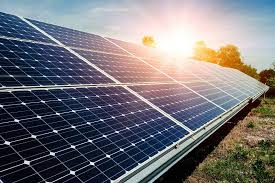
\includegraphics[scale=.4]{Figures/Solar Panels.jpg}}

\date[]{\footnotesize Applied Micro Workshop - \textbf{\today}}
%--------- START DOCUMENT ------------------
\begin{document}
	
\begin{frame}{\titlepage}\end{frame}
\begin{frame}{\frametitle{Presentation Outline}\tableofcontents}\end{frame}
%--------- INTRODUCTION ----------------------
\section{Background and Introduction}


% \begin{frame}
% 	\frametitle{Solar Panel}
%  \begin{itemize}
%  \item Solar power is crucial to clean energy revolution, cost effective way to produce renewable energy
%  %\pause
%  \item In 100\% decarbonization scenarios by 2050, 50\% of energy from solar %according to IEA
%  \end{itemize}
%      \begin{figure}
%         \centering
%         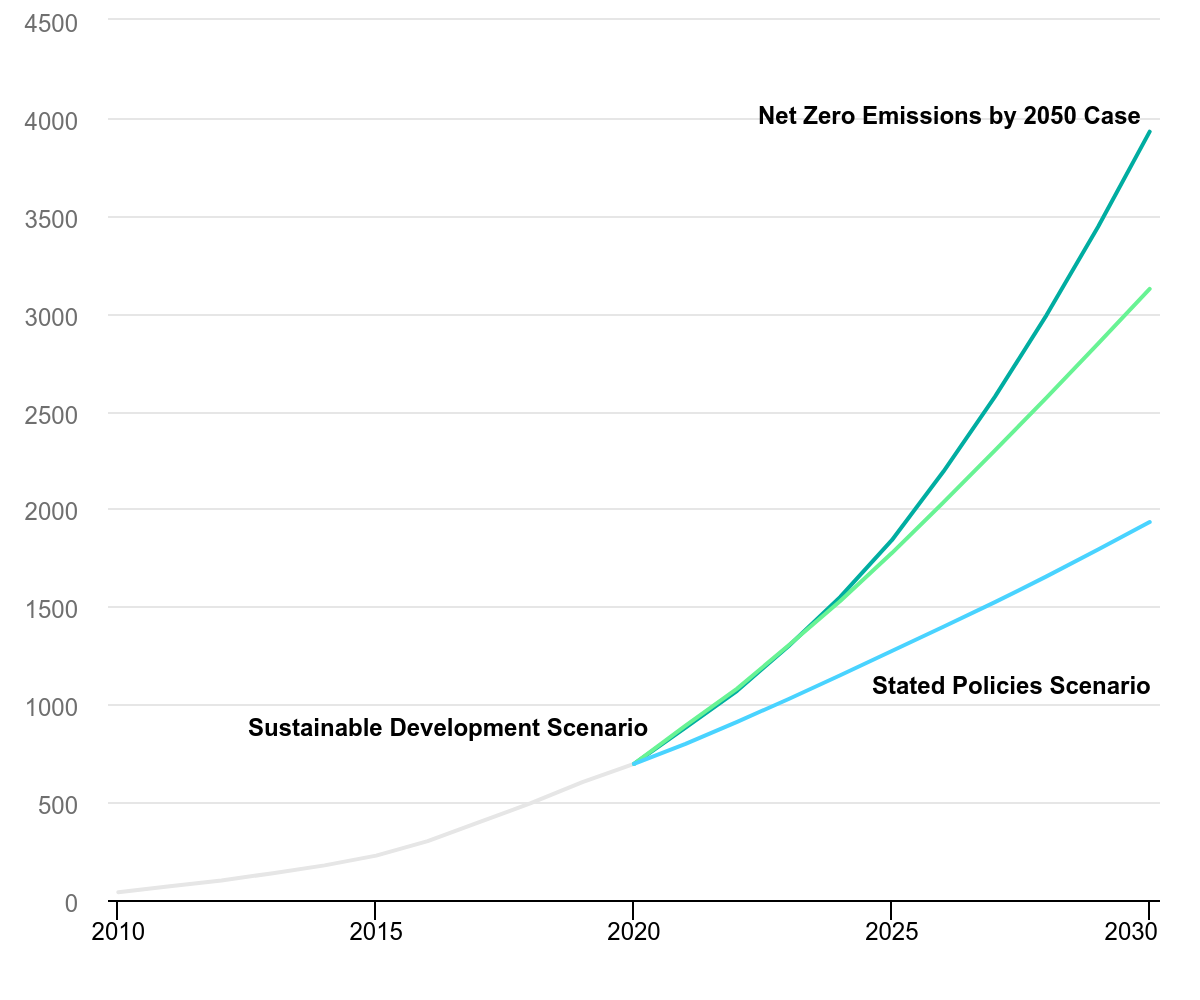
\includegraphics[width=0.4\linewidth]{Figures/Solar Projections by Scenario.png}
%         \caption{GW installed by scenario. Source: IEA}
%         \label{fig:enter-label}
%     \end{figure}
% \end{frame}

% \begin{frame}[plain, noframenumbering]
% \begin{center} 
% {\color{sbured}\LARGE I(i). Overlook of Solar Panel Industry}
% \end{center}
% \end{frame}


\begin{frame}
\frametitle{Overview of Solar Panel Industry}
\begin{enumerate}
    \item Installed solar energy capacity and production increase exponentially; meanwhile, price falls dramatically
    \item China has become dominant in solar panel demand and production during 2006-2013
    %\item Two technologies in production: polysilicon v.s. thin film
    %\item Upstream industrial policies: input price falls substantially
    \item Heavily subsidized industry on both demand, supply, and inputs
    \item Environmental benefits of solar energy and pollution from production
\end{enumerate}
\end{frame}




\begin{frame}{[1] Installed capacity increases exponentially}
    \begin{figure}
        \centering
        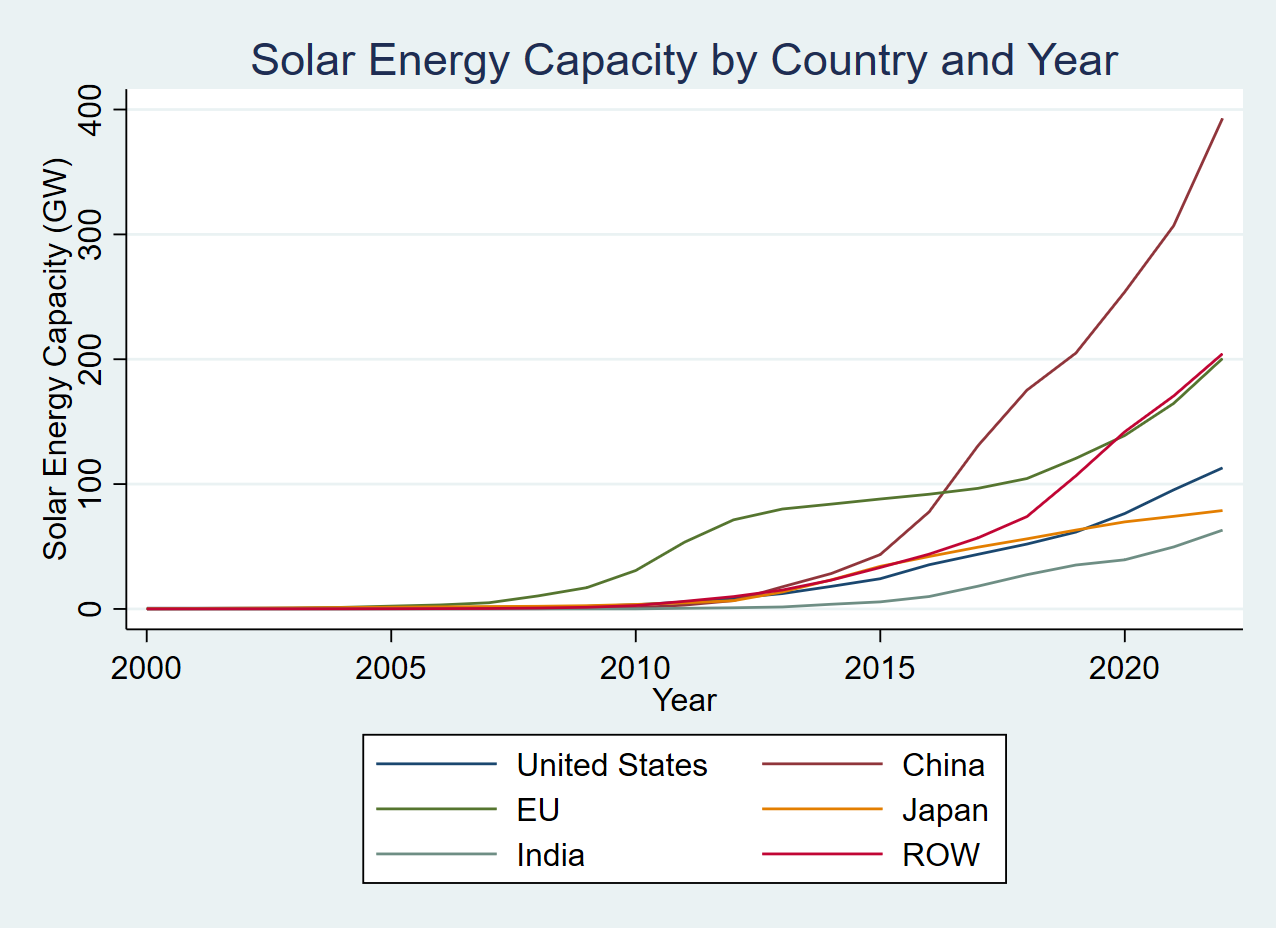
\includegraphics[width=0.75\linewidth]{Figures/Solar Energy Capacity by Country and Year.png}
        %\caption{Solar panel installations increased exponentially since 2000.}
        %\label{fig:enter-label}
    \end{figure}
\end{frame}

\begin{frame}{[1] Price falls dramatically}
    \begin{figure}
        \centering
        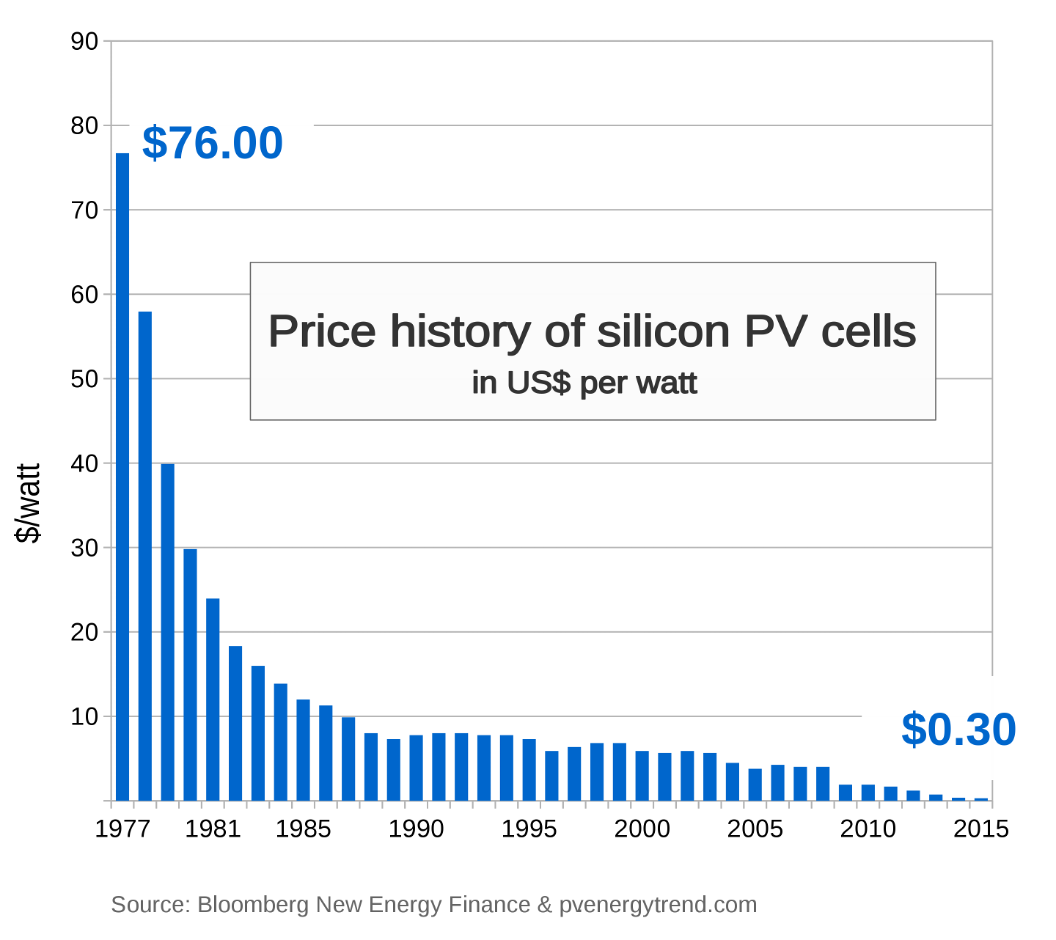
\includegraphics[width=0.6\linewidth]{Figures/price_1977_2013.png}
        %\caption{Solar panel modules have fallen in price over time}
    \end{figure}
\end{frame}

\begin{frame}{[1] Production Explodes}
    \begin{figure}
\centering
    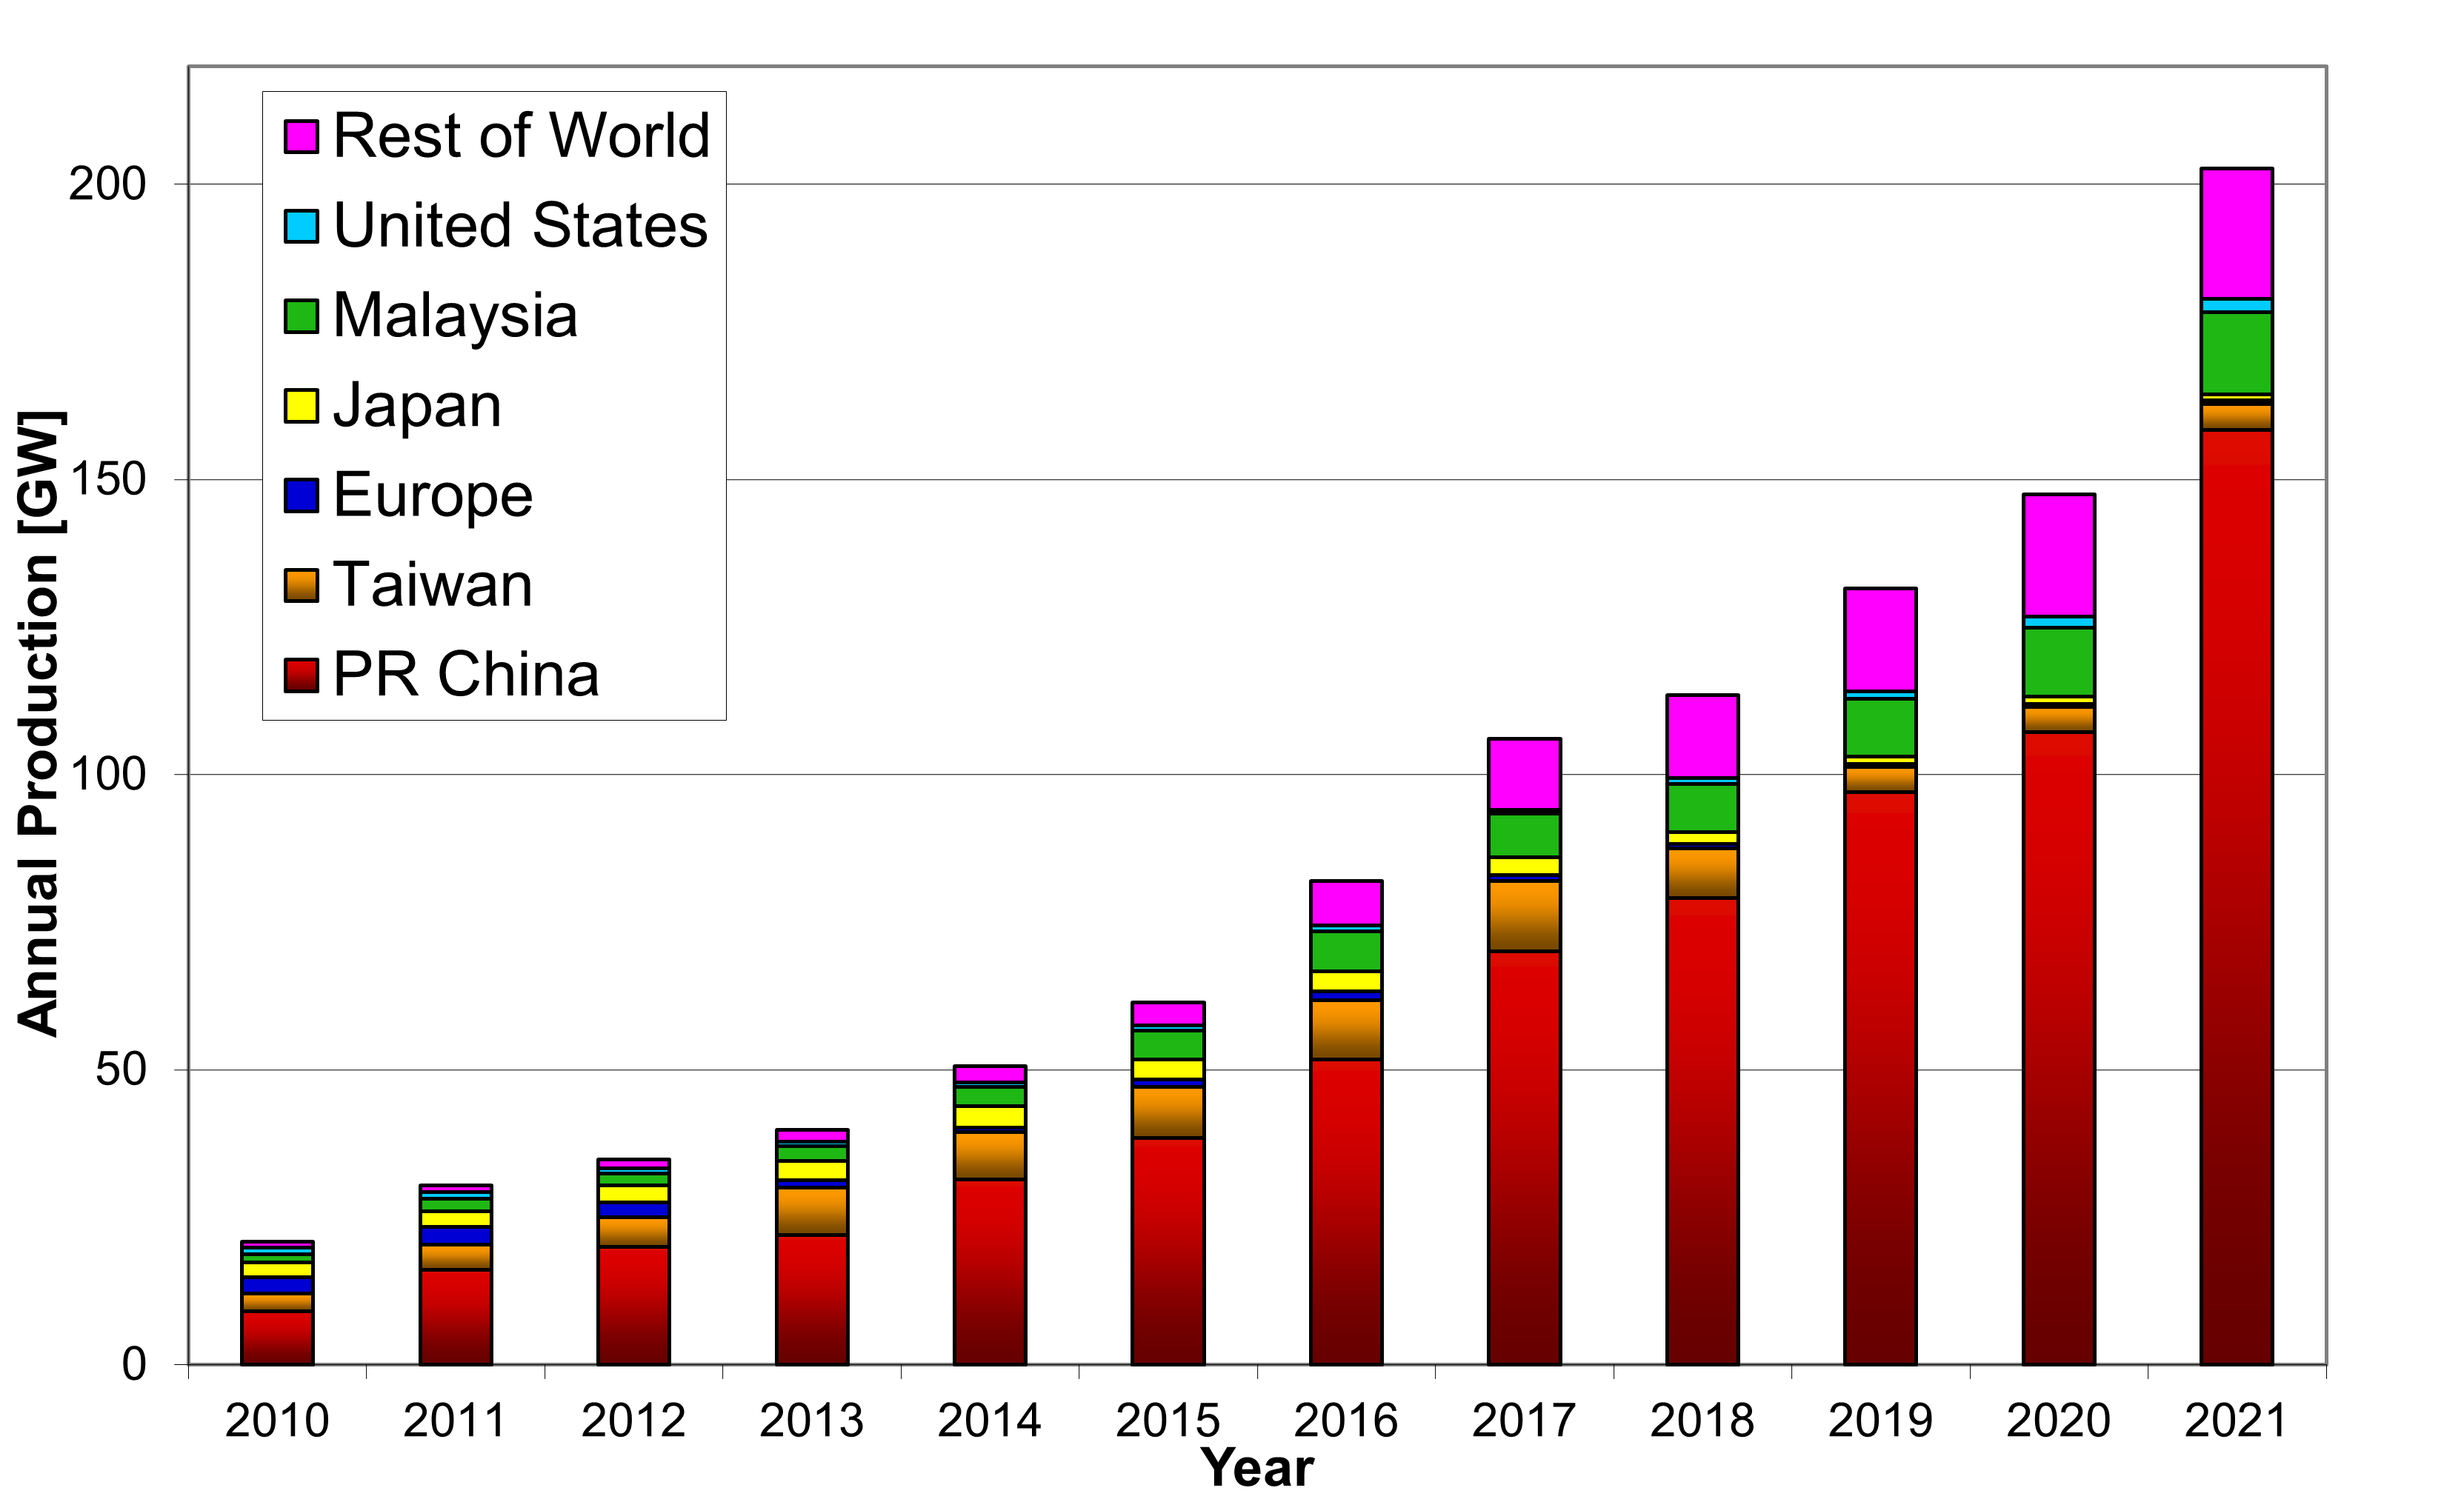
\includegraphics[width=0.8\textwidth]{Figures/Solar Production Growth Over Time.png}
    %\caption{China has become dominant in solar panel manufacturing. Source: Helveston, He, and Davidson (2023)}
     \end{figure}
\end{frame}

\begin{frame}{[2] China has Become Dominant in Production during 2006-2013}
    \begin{figure}
\centering
    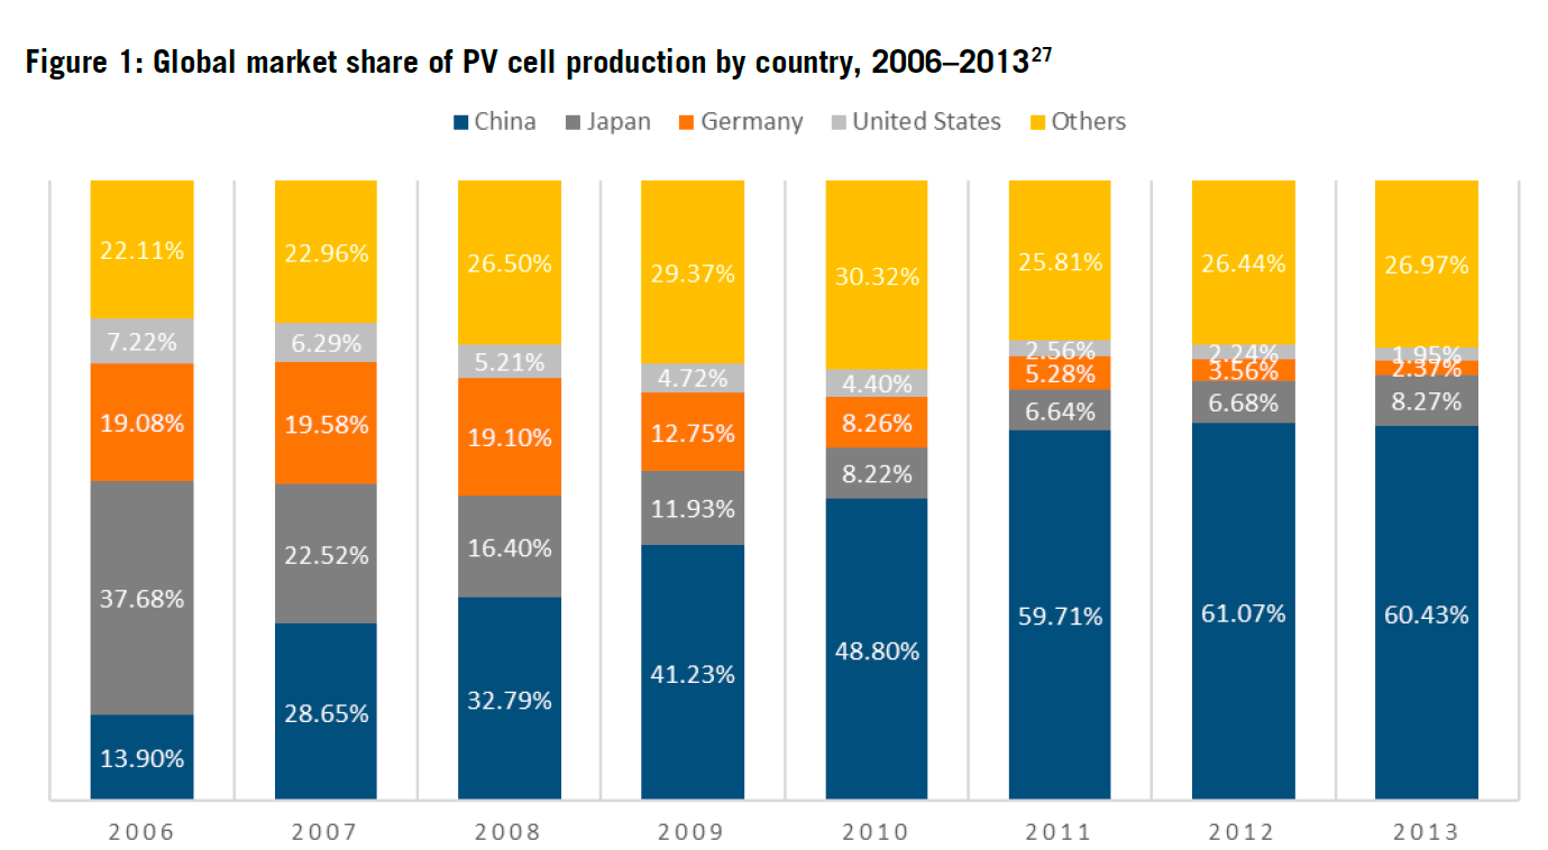
\includegraphics[width=0.8\textwidth]{Figures/production_2006_2013.png}
     \end{figure}
\end{frame}

% \begin{frame}{[4] Two technologies in production}
%    \begin{figure}
%         \centering
%         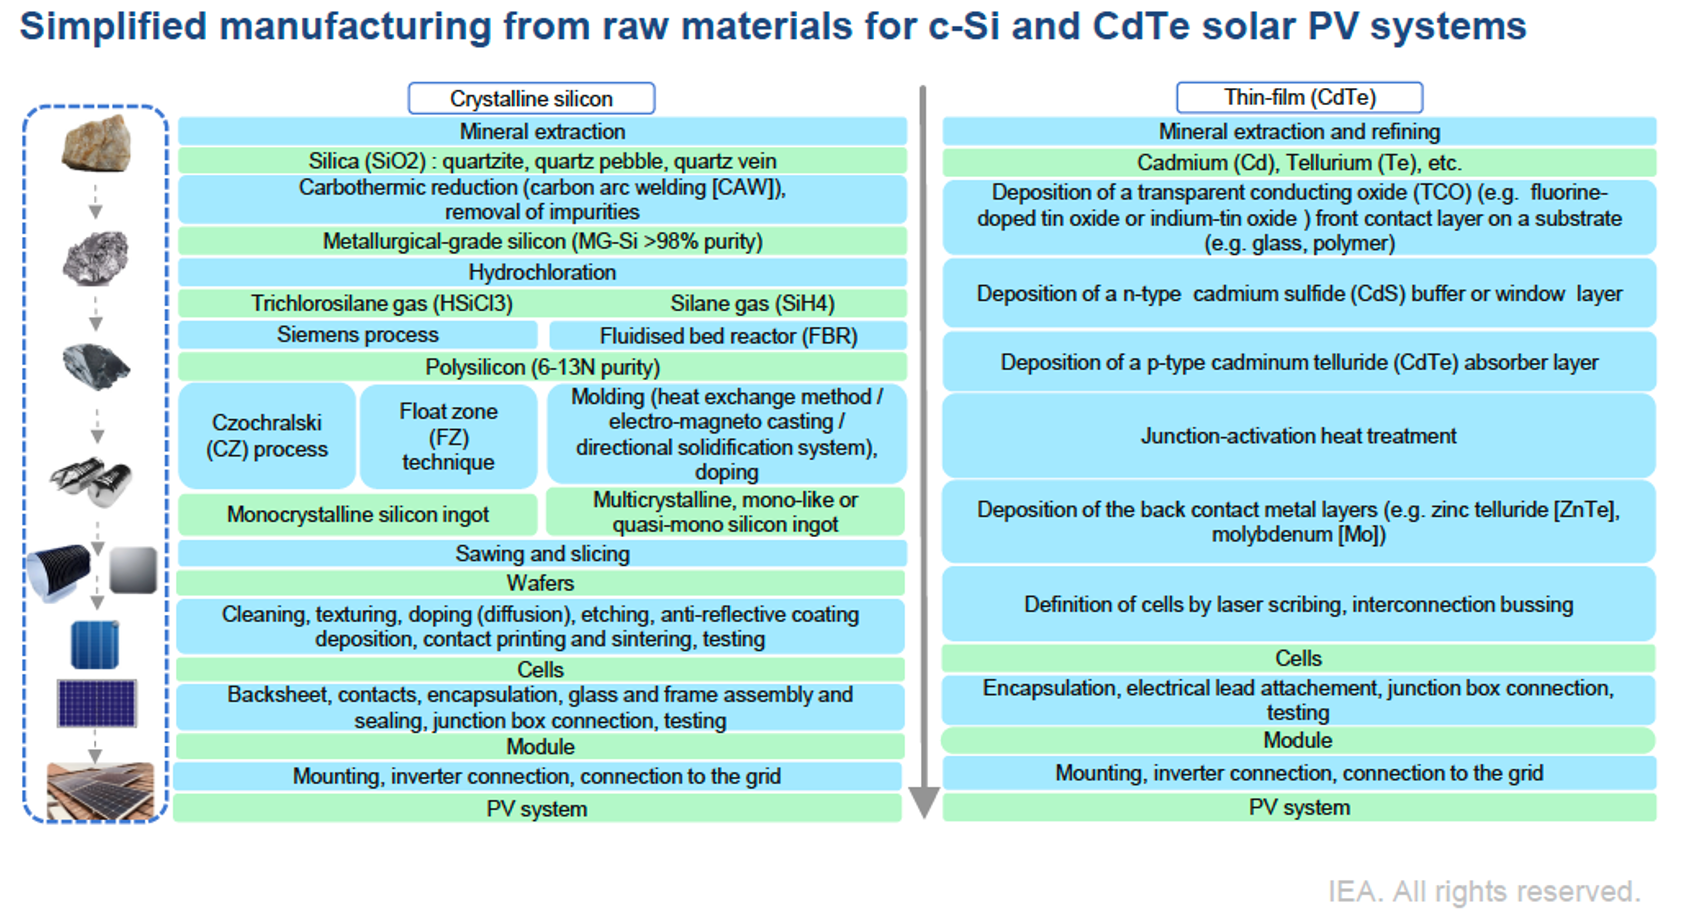
\includegraphics[width=0.9\linewidth]{Figures/two_tech_description.png}
%     \end{figure}
% \end{frame}

% \begin{frame}{[4] Efficiency: Polysilicon v.s. Thin Film}
%    \begin{figure}
%         \centering
%         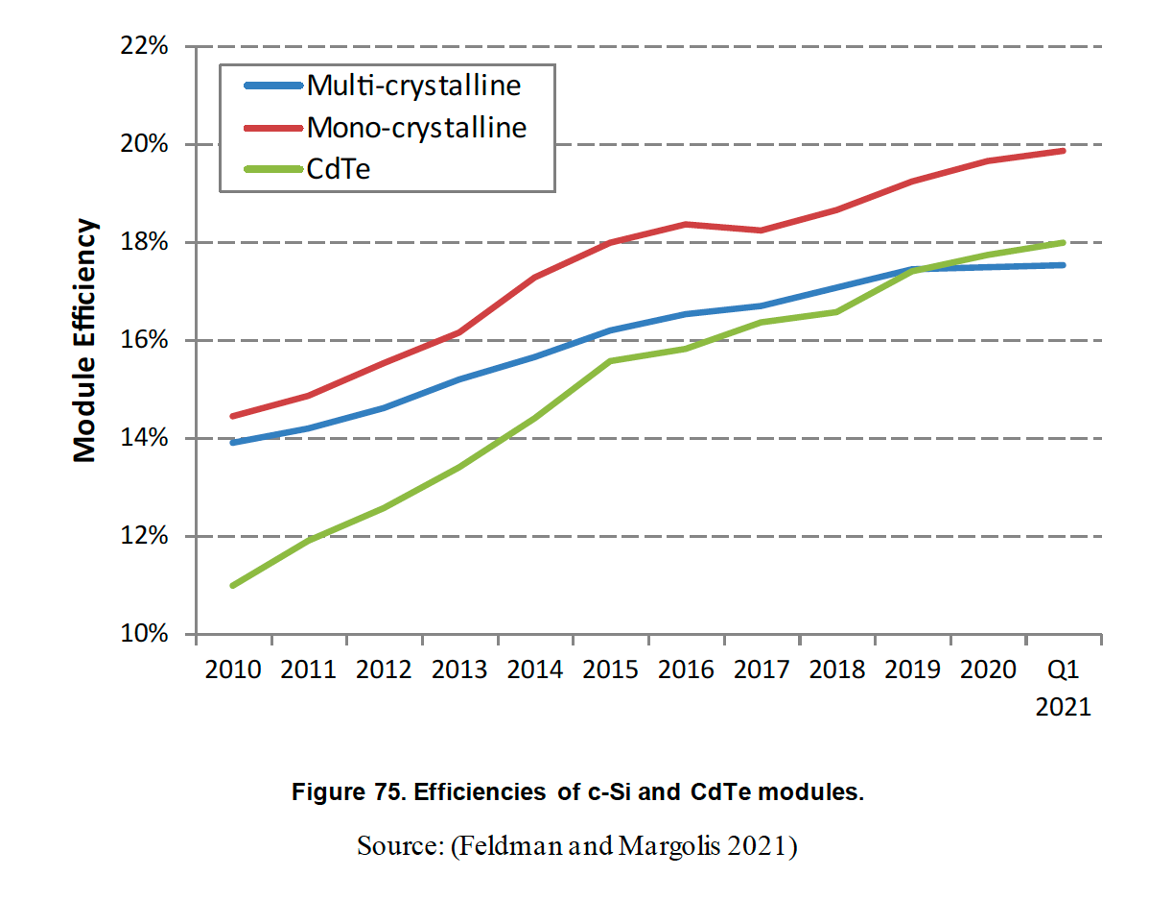
\includegraphics[width=0.7\linewidth]{Figures/two_tech_efficiency.png}
%     \end{figure}
% \end{frame}

% \begin{frame}{[4] Production Share: Polysilicon v.s. Thin Film}
%    \begin{figure}
%         \centering
%         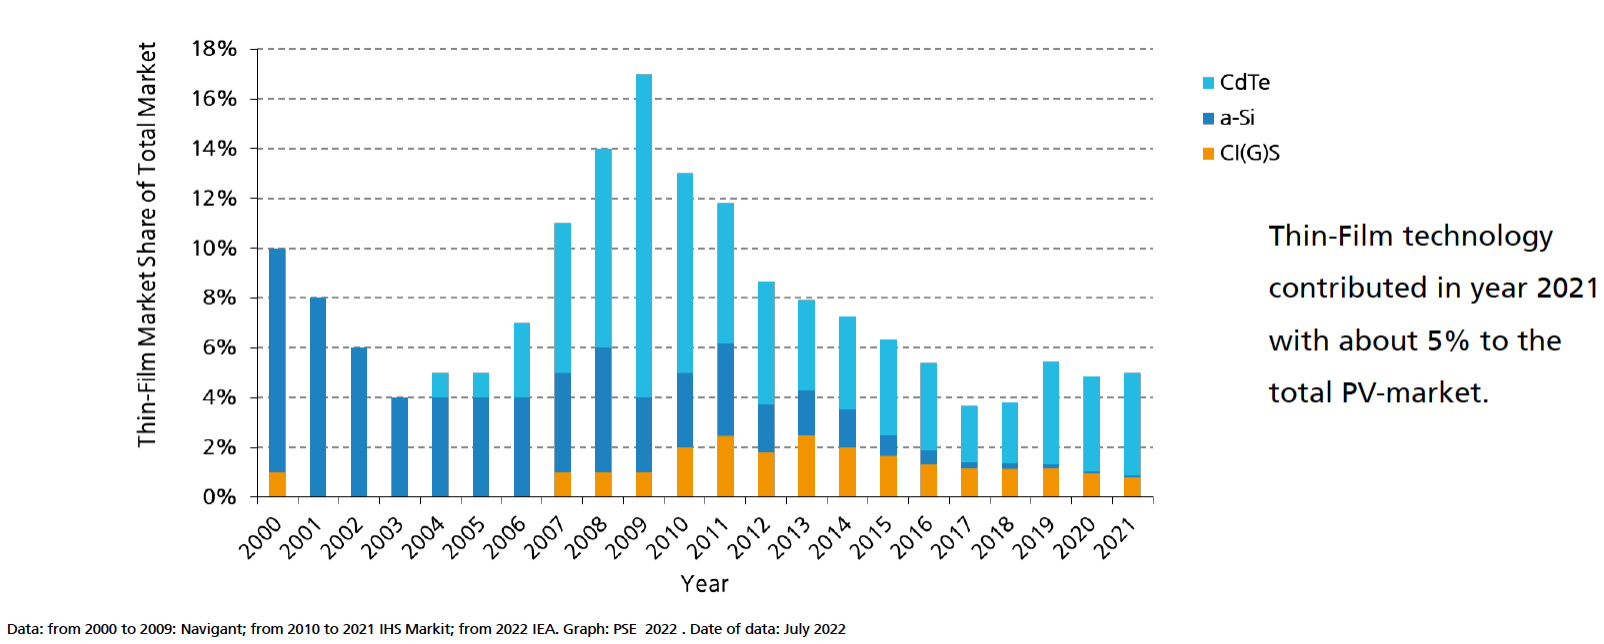
\includegraphics[width=1.0\linewidth]{Figures/two_tech_share_2000_2021.png}
%     \end{figure}
% \end{frame}

\begin{frame}{[3] Industrial Policies: Worldwide}
\begin{itemize}
    \item Demand Side:
    \begin{itemize}
        \item Tax credits, feed-in tariff, etc.
     \end{itemize}
    \item Production Side:
    \begin{itemize}
        \item Production cost: tax credits or exemptions, lower energy price, funds to reduce labor costs through lower charges, etc.
        \item Entry cost: grants and low-cost or free land, funds for R\&D or for small firms
        \item Investment cost: preferential loans, etc.
     \end{itemize}
\end{itemize}
    %\begin{figure}
    %    \centering
    %    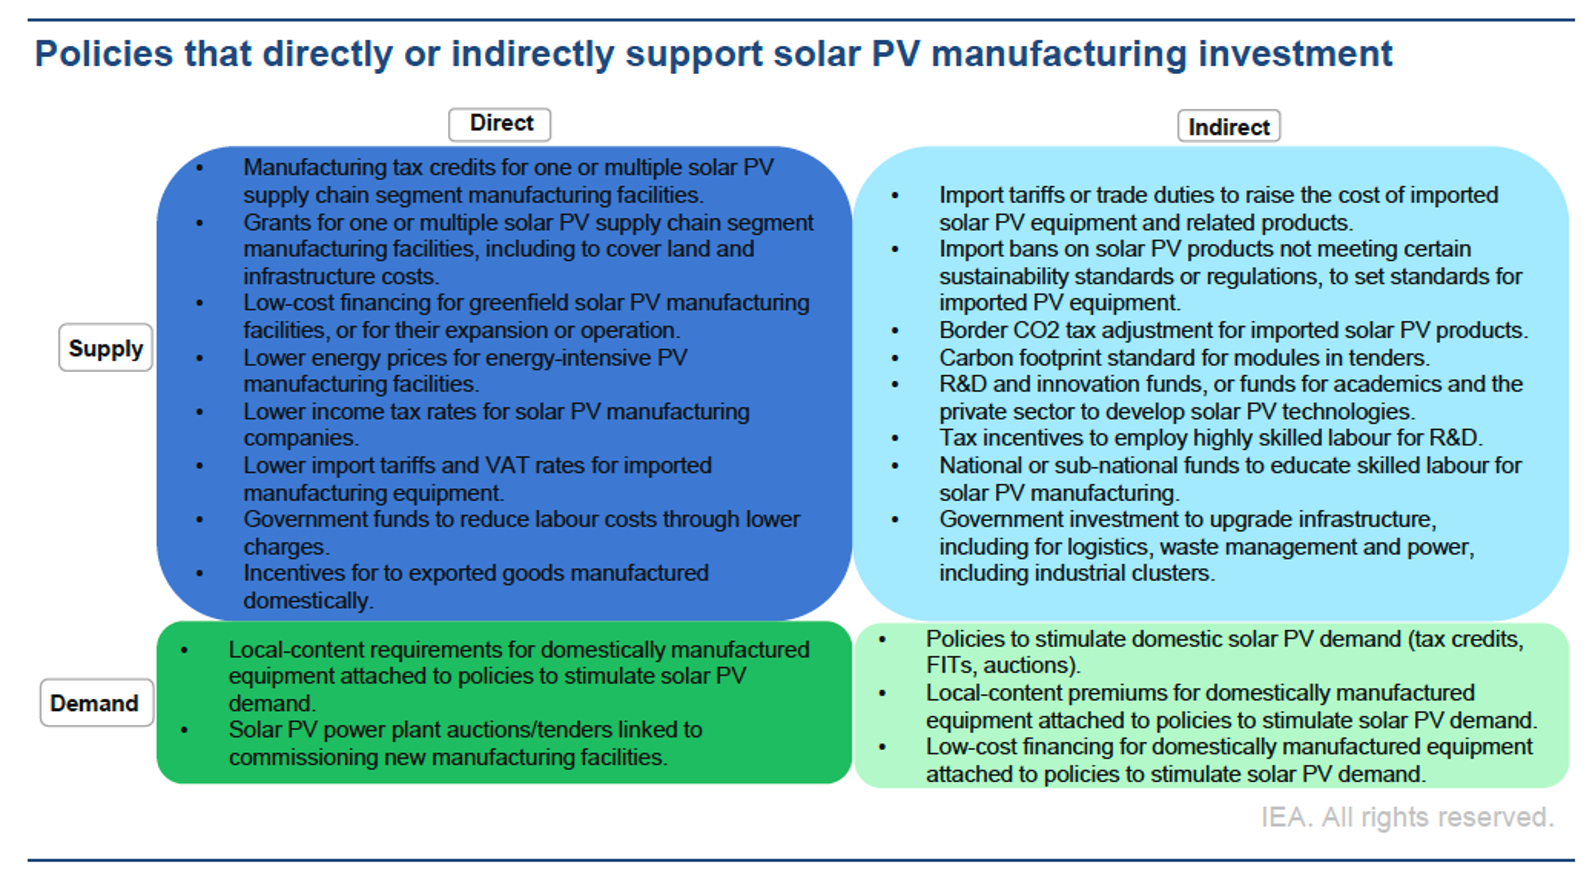
\includegraphics[width=0.9\linewidth]{Figures/policies_PV.png}
   % \end{figure}
\end{frame}

\begin{frame}{[3] Industrial Policies: China}
    \begin{itemize}
        \item Demand and production: similar as other countries
            \begin{itemize}
            \item Example: the Golden Sun program (introduced by China in 2009)
            \end{itemize}
        \item Subsidies on Polysilicon (Input) Production
        \item White list of firms (2009)
    \end{itemize}
\end{frame}

%\begin{frame}{[4] Policies on demand and production: China}
%    \begin{figure}
%        \centering
%        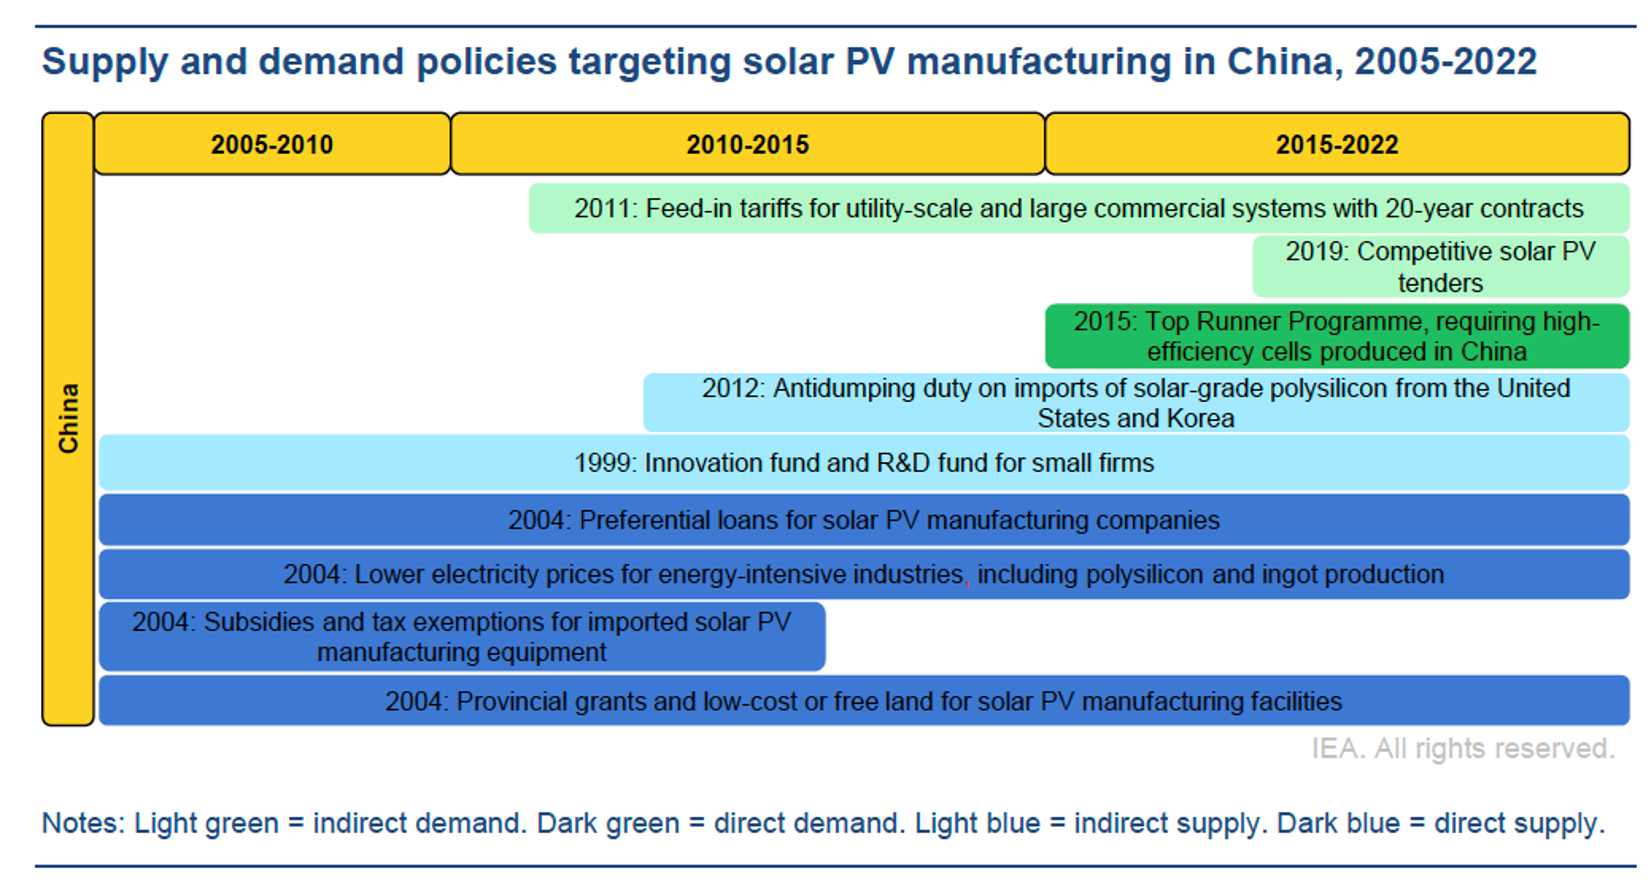
\includegraphics[width=0.9\linewidth]{Figures/policies_China.png}
%    \end{figure}
%\end{frame}

\begin{frame}{[3] Polysilicon Production over Time}
    \begin{figure}
        \centering
        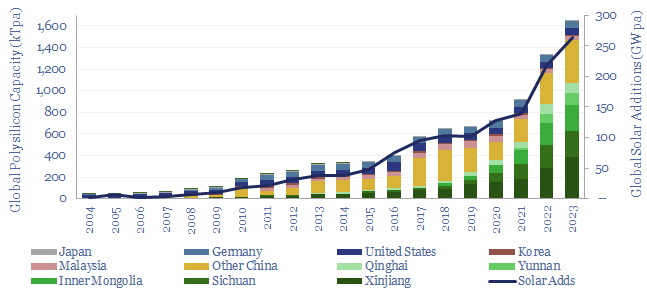
\includegraphics[width=0.9\linewidth]{Figures/Global-polysilicon-production.png}
    \end{figure}
\end{frame}

\begin{frame}{[3] China's Share in Polysilicon Production}
    \begin{figure}
        \centering
        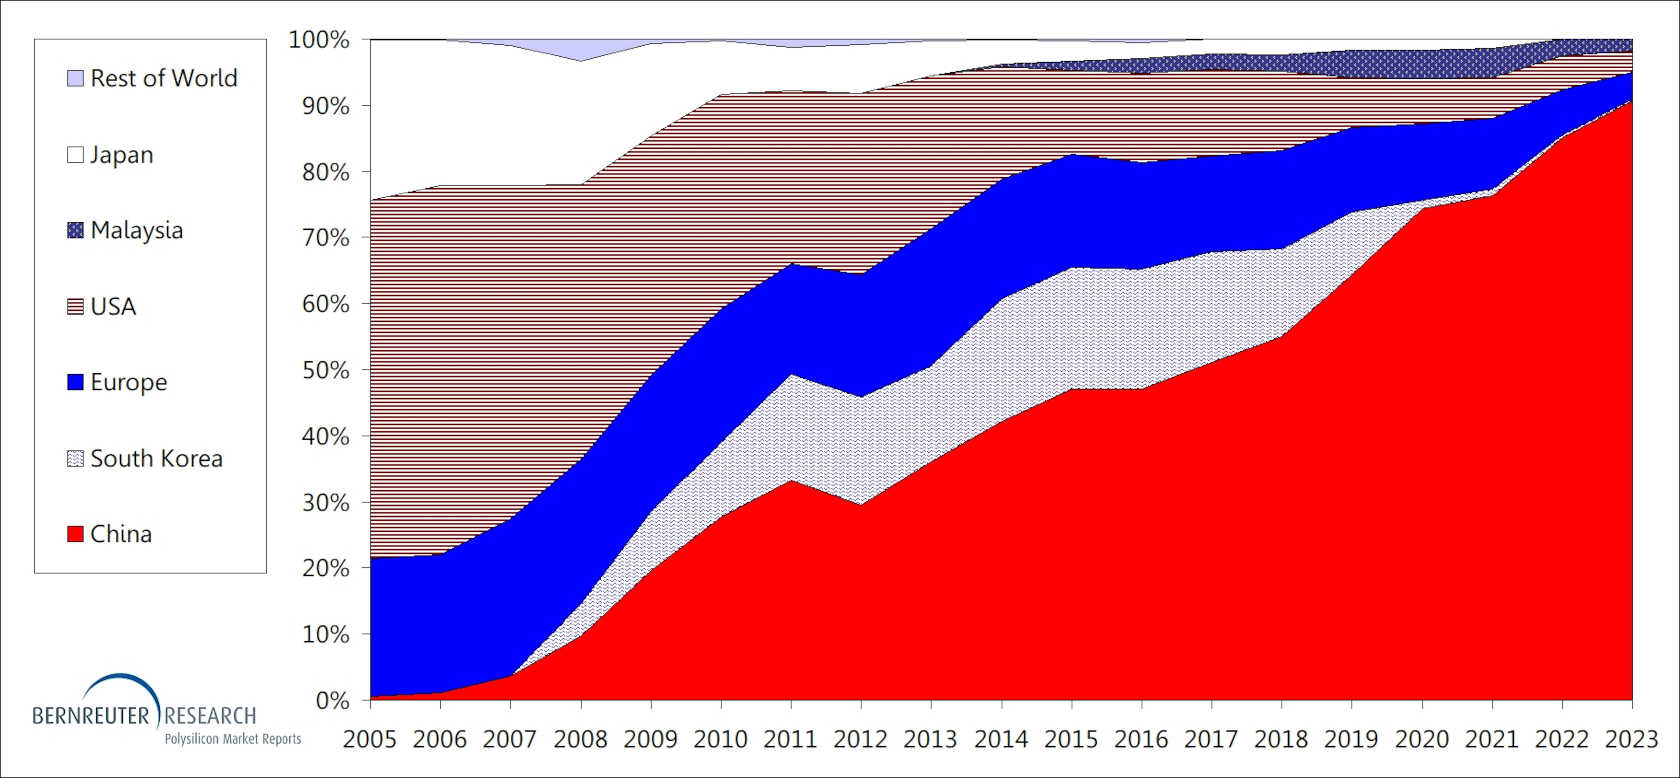
\includegraphics[width=0.9\linewidth]{Figures/polysilicon-market-shares-by-country-2005-2023.jpg}
    \end{figure}
\end{frame}

% \begin{frame}{[5] Polysilicon production by country}
%     \begin{figure}
%         \centering
%         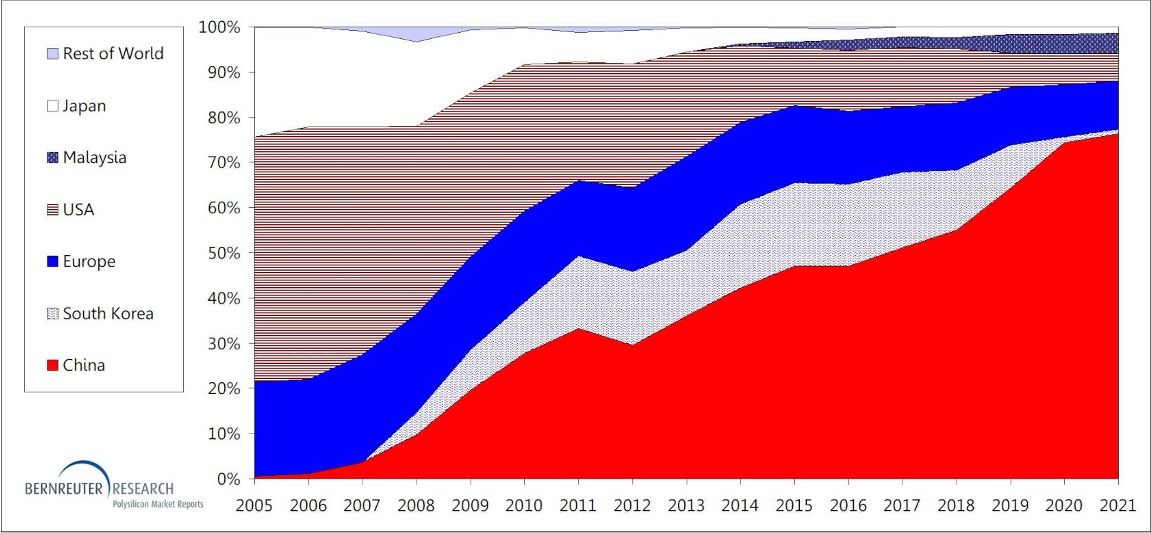
\includegraphics[width=0.9\linewidth]{Figures/polysilicon_production_country.jpg}
%     \end{figure}
% \end{frame}


\begin{frame}{[3] Polysilicon Price over Time}
    \begin{figure}
        \centering
        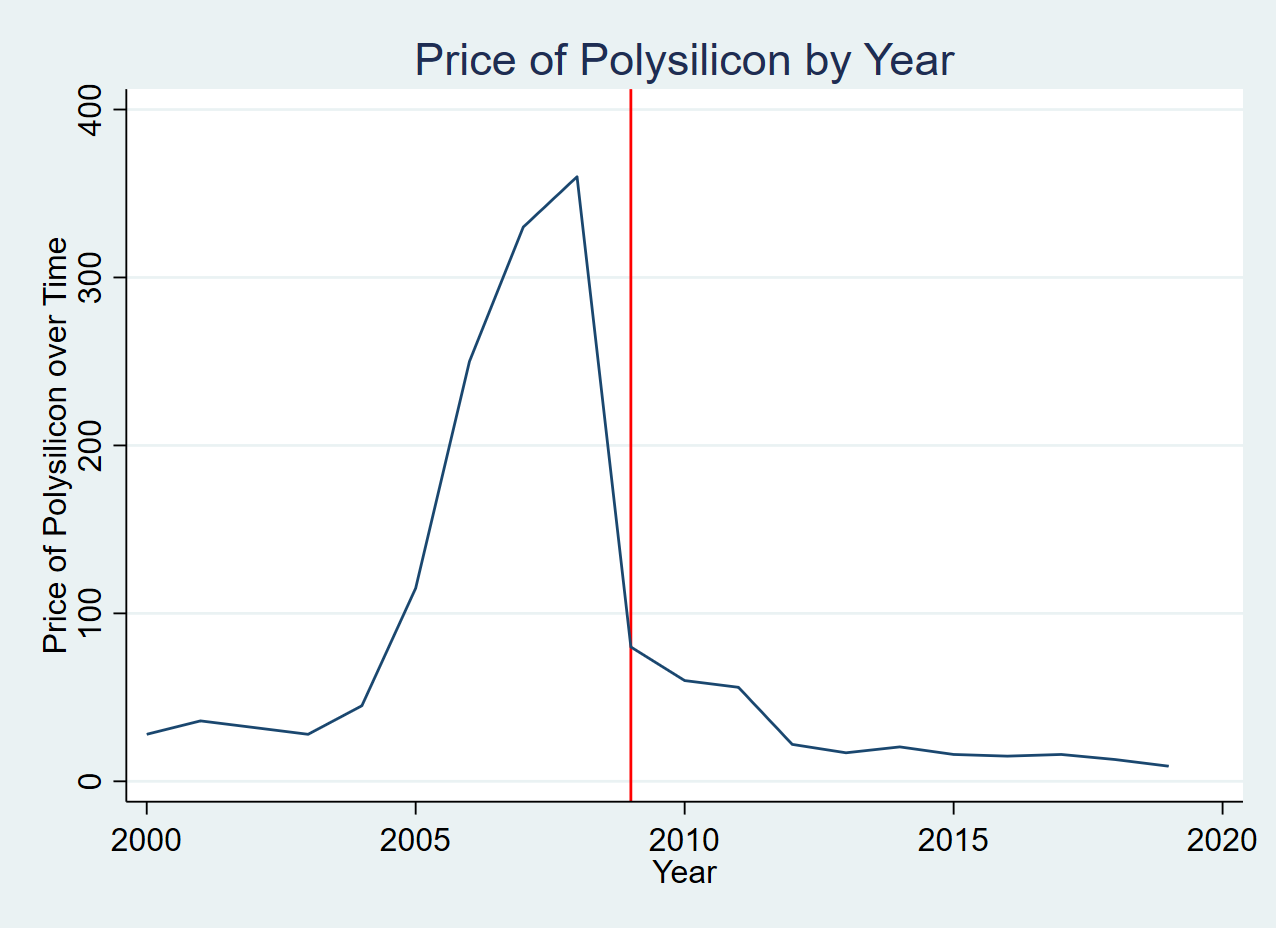
\includegraphics[width=0.75\linewidth]{Figures/Price of Polysilicon over Time.png}
       % \caption{China has dramatically subsidized polysilicon production}
    \end{figure}
\end{frame}

% \begin{frame}{[5] Polysilicon demand: semiconductor v.s. PV}
%     \begin{figure}
%         \centering
%         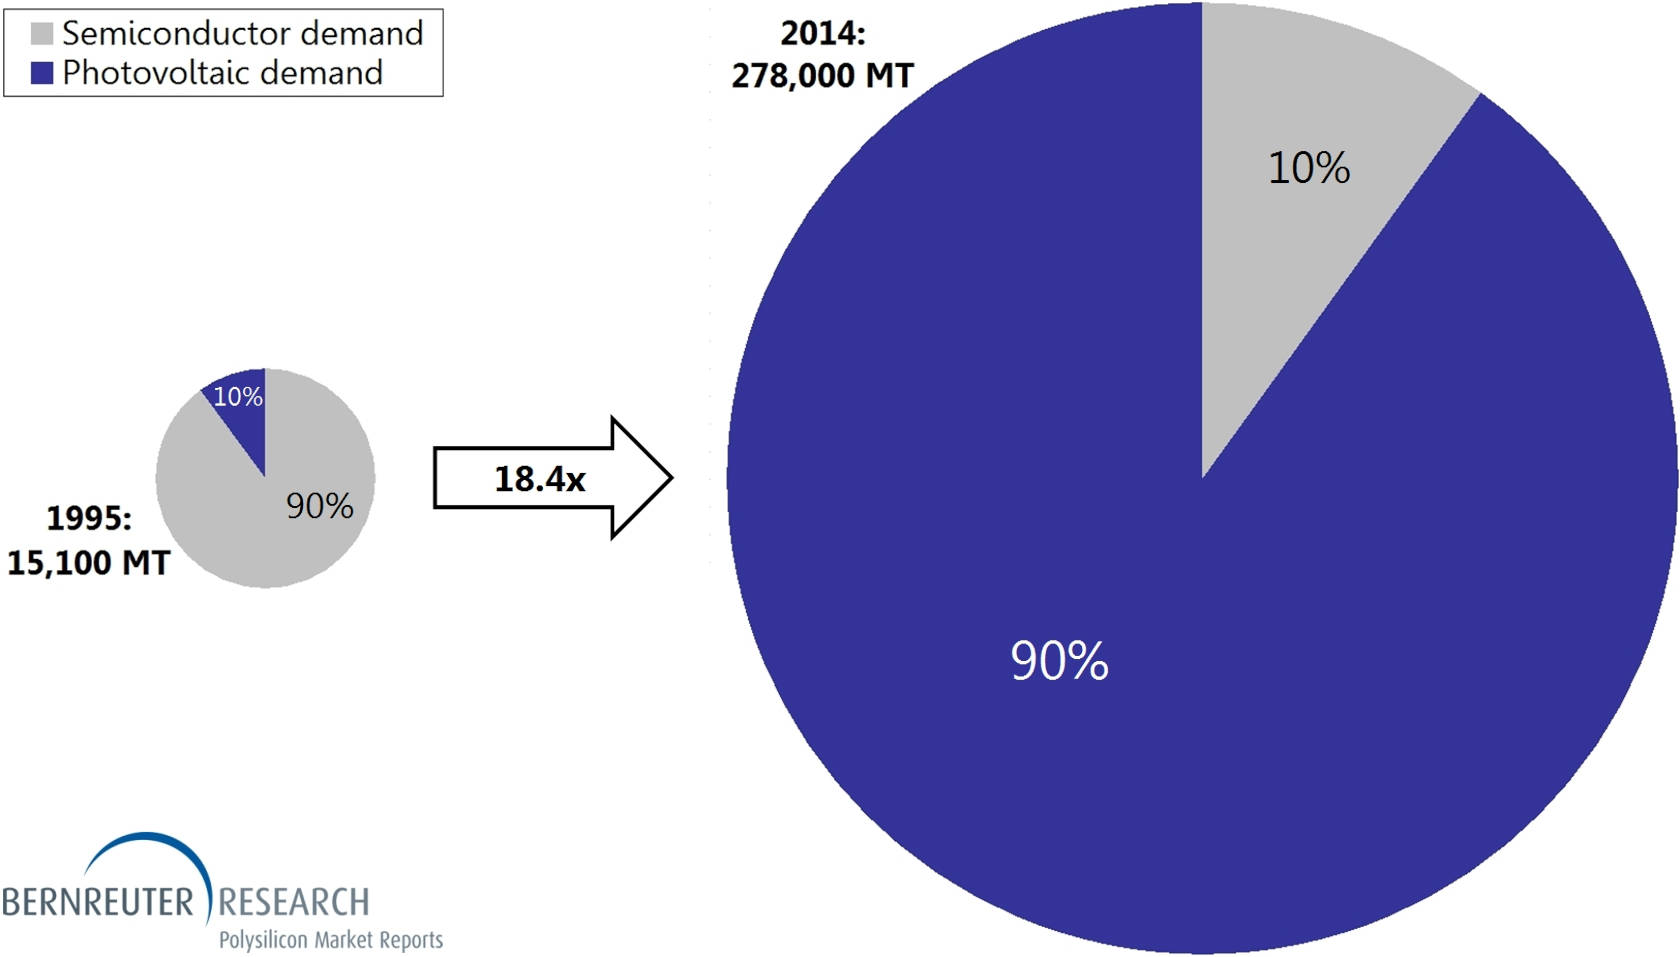
\includegraphics[width=0.75\linewidth]{Figures/polysilicon-demand-solar-semiconductor-shares-1995-2014.jpg}
%     \end{figure}
% \end{frame}


\begin{frame}{[3] Entry and Exits of Chinese  Firms}
   \begin{figure}
    \centering
   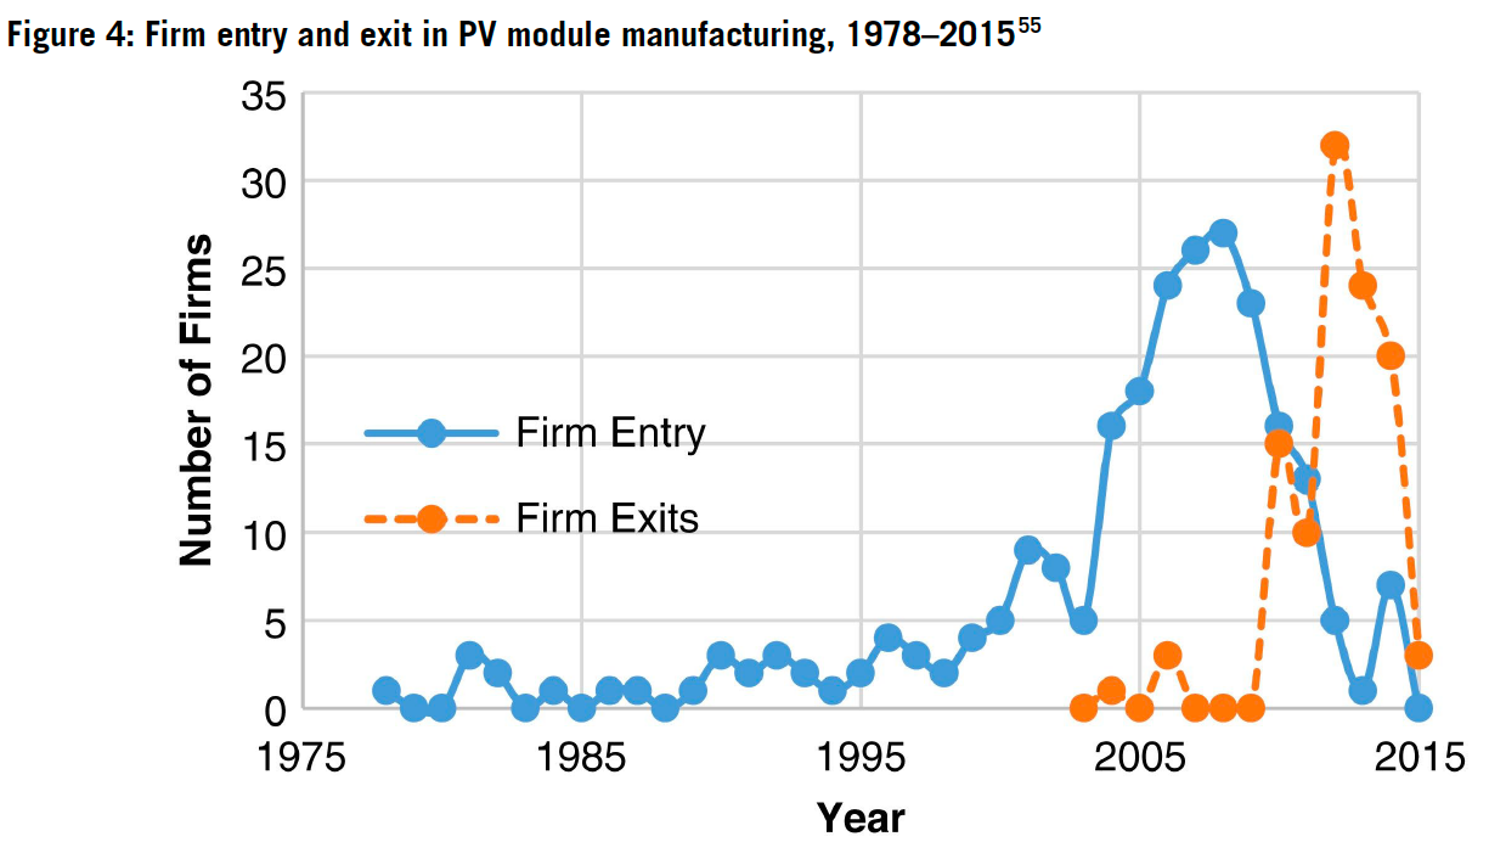
\includegraphics[width=0.8\textwidth]{Figures/entry_exit_1975_2015.png}
    \end{figure}
\end{frame}

\begin{frame}{[4] Environmental Benefits of Solar Energy}
% \begin{itemize}
%  \item In 100\% decarbonization scenarios by 2050, 50\% of energy from solar %according to IEA
%  \end{itemize}
%      \begin{figure}
%         \centering
%         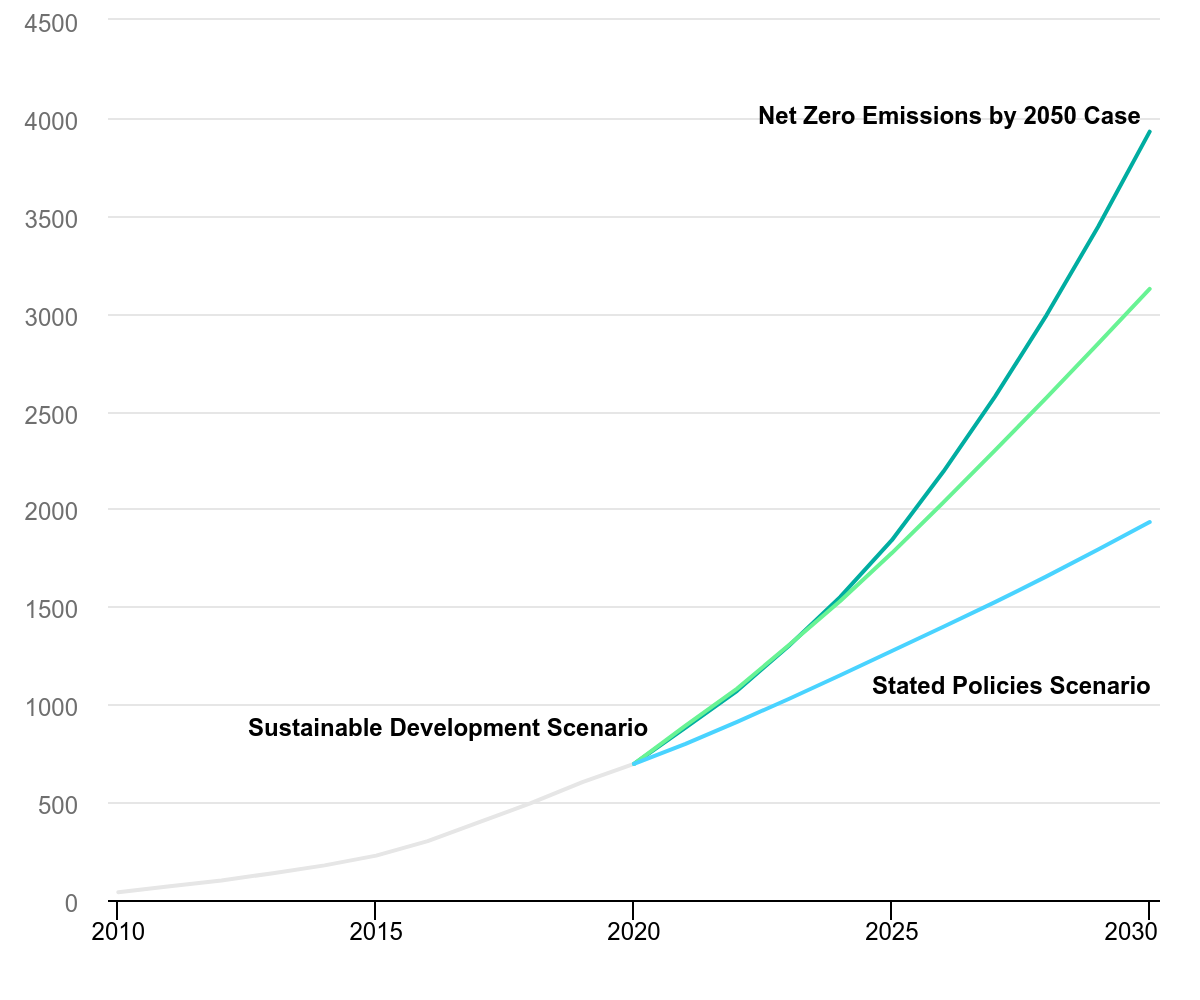
\includegraphics[width=0.6\linewidth]{Figures/Solar Projections by Scenario.png}
%         \caption{GW installed by scenario. Source: IEA}
%     \end{figure}
\begin{itemize}
    \item No air pollution or green house gases when operating
    \pause
    \item Positive environmental gain when solar energy replaces or reduces the use of other energy sources
    \pause
    \item How much gain of solar energy in a specific location at a specific point of time depends on the energy sources used in that location and at that point of time
    \begin{itemize}
        \item The benefit is larger if the energy replaced by solar is relatively dirty (e.g., coal) 
    \end{itemize}
\end{itemize}
\end{frame}

\begin{frame}{[4] PV Production: Emissions}
    \begin{figure}
        \centering
        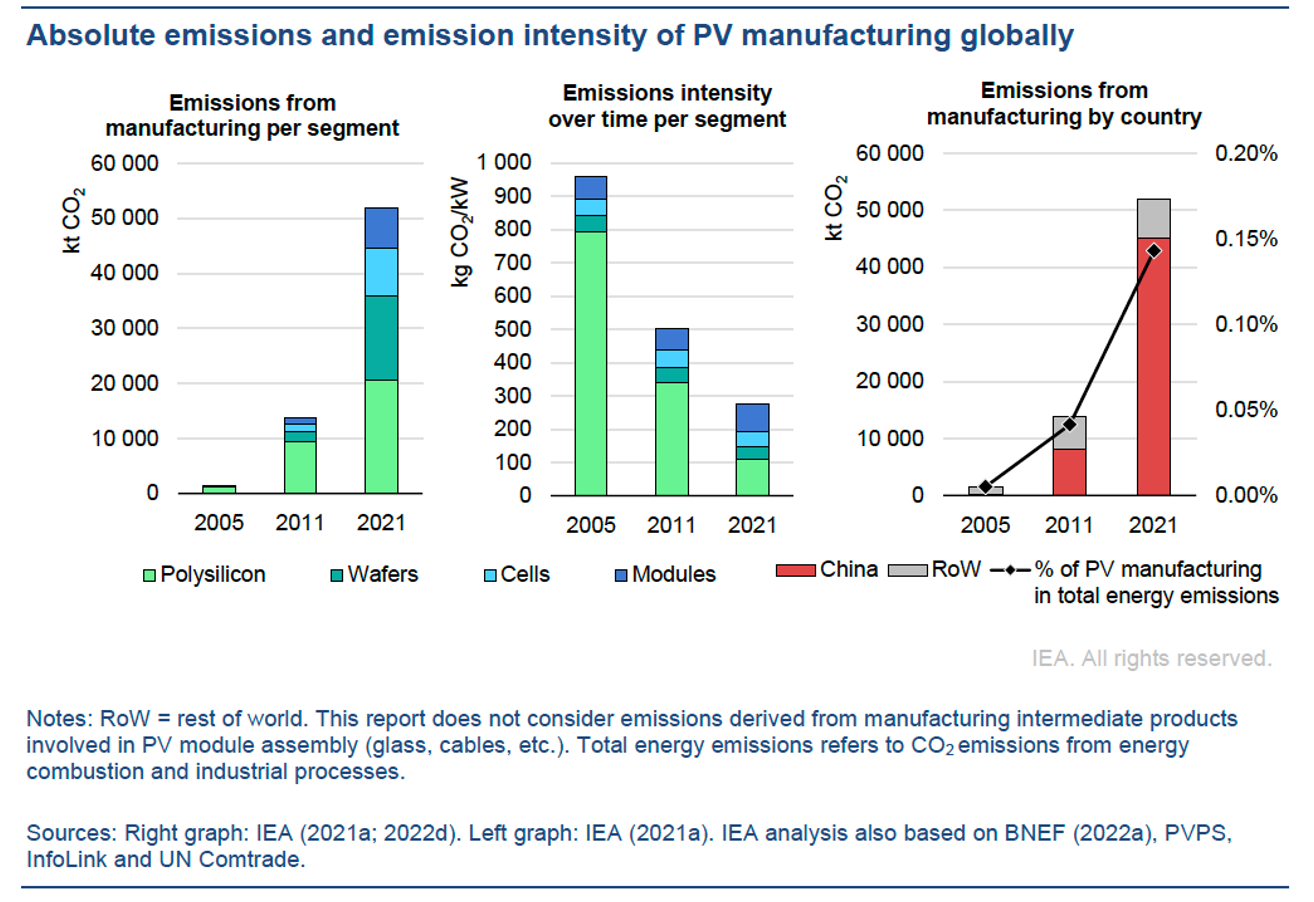
\includegraphics[width=0.75\linewidth]{Figures/emissions_PV_production_country.png}
    \end{figure}
\end{frame}

\begin{frame}{[4] PV production: Electricity Use}
    \begin{figure}
        \centering
        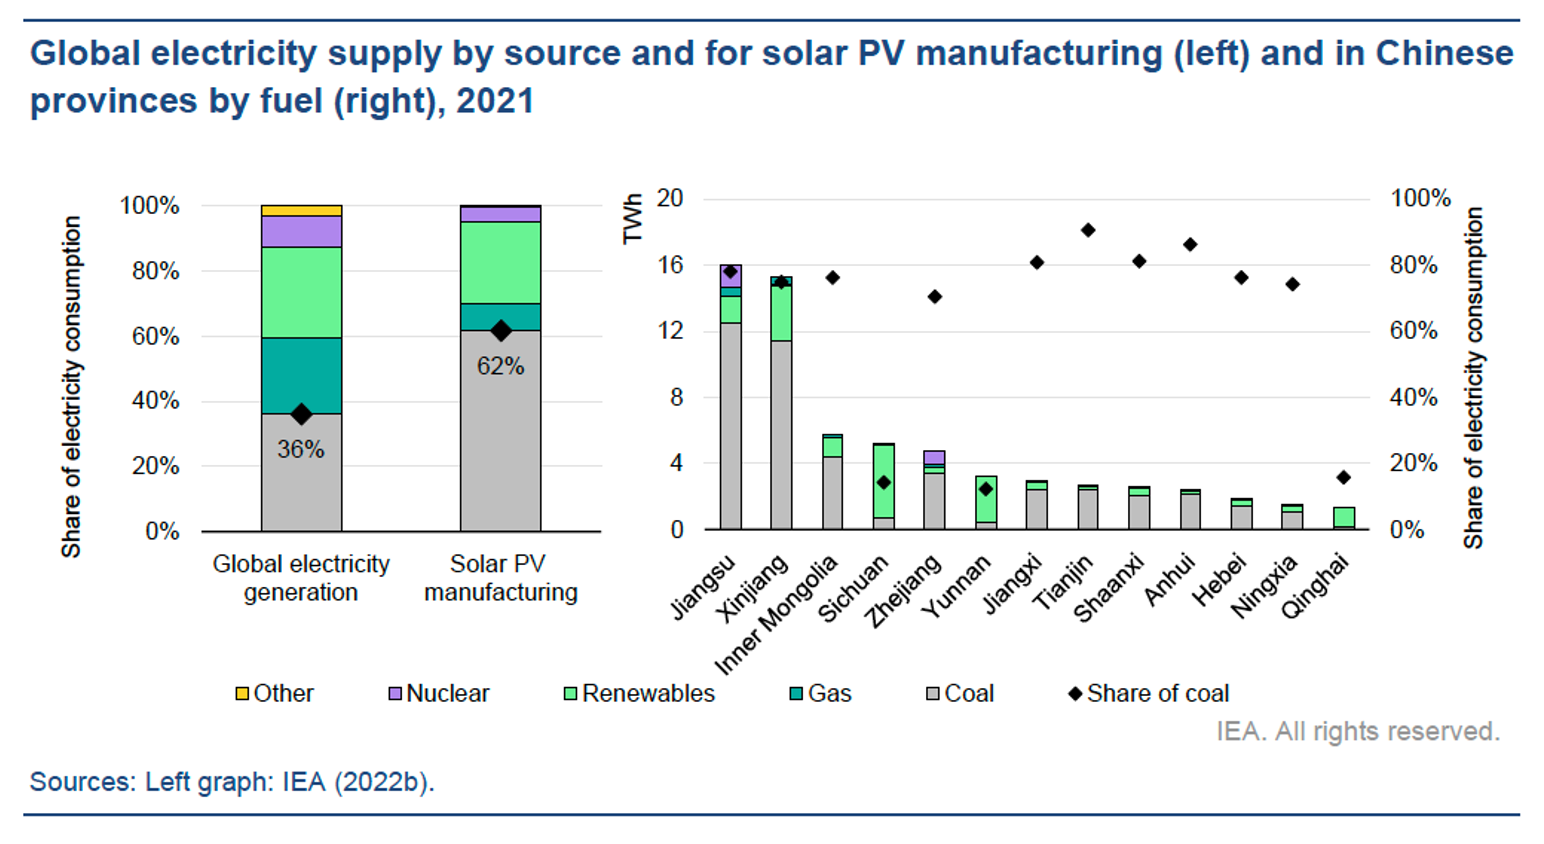
\includegraphics[width=0.75\linewidth]{Figures/electricity_sources_PV_production.png}
    \end{figure}
\end{frame}
% \begin{frame}{Solar Industrial Policy China}
%     \begin{enumerate}
%         \item Demand subsidy
%         \begin{itemize}
%         \item Golden sun program
%         \item feed-in tariff
%         \end{itemize}
%         \pause
%         \item Production subsidies
%         \begin{itemize}
%             \item Subsidies on upstream firms, e.g. polysilicon
%             \item Tax breaks by province
%         \end{itemize}
%         \pause
%         \item Investment subsidies:
%         \begin{itemize}
%             \item Low-interest loans for solar panel firms
%         \end{itemize}
%         \pause
%         \item Entry and exit subsidies: 
%         \begin{itemize}
%             \item Low rent prices for solar panel firms
%         \end{itemize}
%     \end{enumerate}
% \end{frame}

\begin{frame}[plain, noframenumbering]
\begin{center} 
{\color{sbured}\LARGE I(ii). What we do}
\end{center}
\end{frame}

\begin{frame}[label=RQ]
	\frametitle{Research Question}
        \begin{itemize}

        \item Examine the impacts of different industrial policies on
            \begin{itemize}
                \item Equilibrium price \& installation \& production of solar panels
                \item Environmental benefits from installation \& emissions from production: location specific
            \end{itemize}
         \pause
        \item Different industrial policies include
            \begin{itemize}
                \item Demand side: installation subsidies \& tariffs
                \item Production side: production cost, entry cost, investment
                \item Upstream (polysilicon) industrial policies leading to the collapse of input price
            \end{itemize}
        \end{itemize}
\end{frame}

\begin{frame}[label=RQ]
	\frametitle{What we do in this paper}
        \begin{enumerate}
        \item Build a dynamic model of investment, entry, and exit of solar panel manufacturing industry
        \pause
       \item BBL estimation approach to estimate the model by combining different datasets
       \pause
       \item Counterfactuals to quantify the impacts of various industrial policies
       \begin{itemize}
           \item Equilibrium price and output
           \item Location-specific environmental benefits from installation \& emissions from production
       \end{itemize}

        \end{enumerate}
\end{frame}

\begin{frame}{Prior Literature}
    \begin{enumerate}
        \item Industrial policy: 
        \begin{itemize} 
        \item Barwick, Kalouptsidi, and Zahur (2023); Juhász, Lane, and Rodrik  (2020); Goldberg, et. al (2024); Wang and Xing (2024 JMP)
        \item Our paper: 
            \begin{itemize} 
              \item Clean energy industry: Environmental impacts of production and use 
              \item Examine both economic \& environmental impacts
            \end{itemize}
        \end{itemize}
        \pause
        \item Effectiveness of policies on clean energy markets
        \begin{itemize} 
        \item Mainly focus on demand subsidies: Bayaliyev, Kalloz, and Robinson (2011);  Zhang et al. (2022); Yang et al. (2021); Li et al. (2017)
        \item Our paper: demand + supply side + upstream industrial policies
        \end{itemize}
    \end{enumerate}
\end{frame}

% \section{Data}

% \begin{frame}[plain, noframenumbering]
% \begin{center} 
% {\color{sbured}\LARGE II. Data}
% \end{center}
% \end{frame}

\begin{frame}[label=Data]{Dataset Description}
\begin{enumerate}
    \item Demand side: country-year (quarter) level data on tariffs, prices, installation, demand shifters (World Bank)
    \item Production side:
    \begin{itemize}
        \item Chinese firm-country-year-level trade data: exports volume
        \item Chinese firm-level manufacturing data: Survey data from China's manufacturing survey on firm-specific variables
        \item Region-year level production data
    \end{itemize}

\end{enumerate}
\end{frame}

% \begin{frame}{China's Exports by Country}
%     \begin{figure}
%         \centering
%         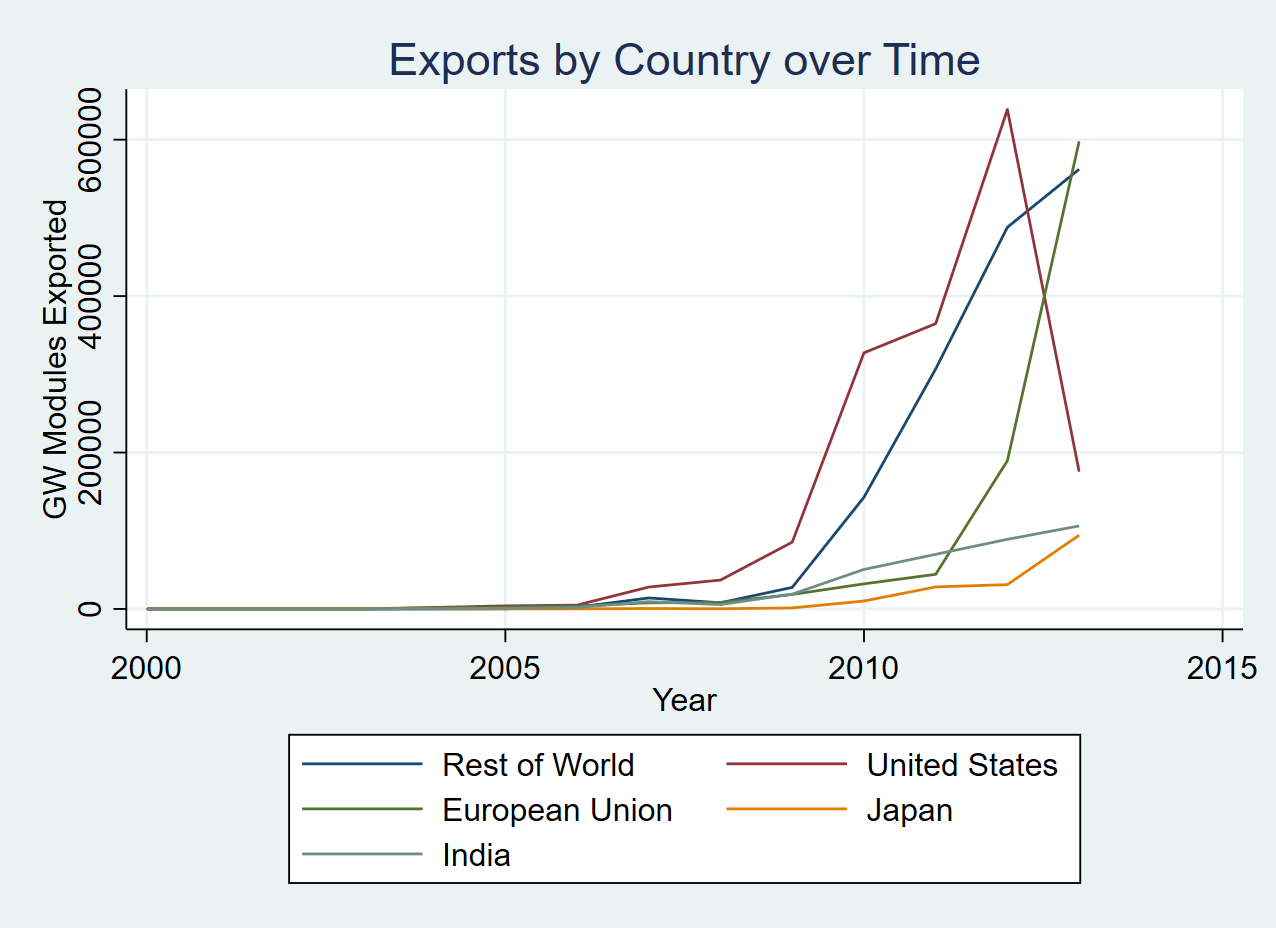
\includegraphics[width=0.75\linewidth]{Figures/Exports by Country by year except China.png}
%        % \caption{China's Exports by Country by Year}
%     \end{figure}
% \end{frame}

% \begin{frame}{Chinese firms: entered quickly at start, then exited relatively quickly}
%     \begin{figure}
%         \centering
%         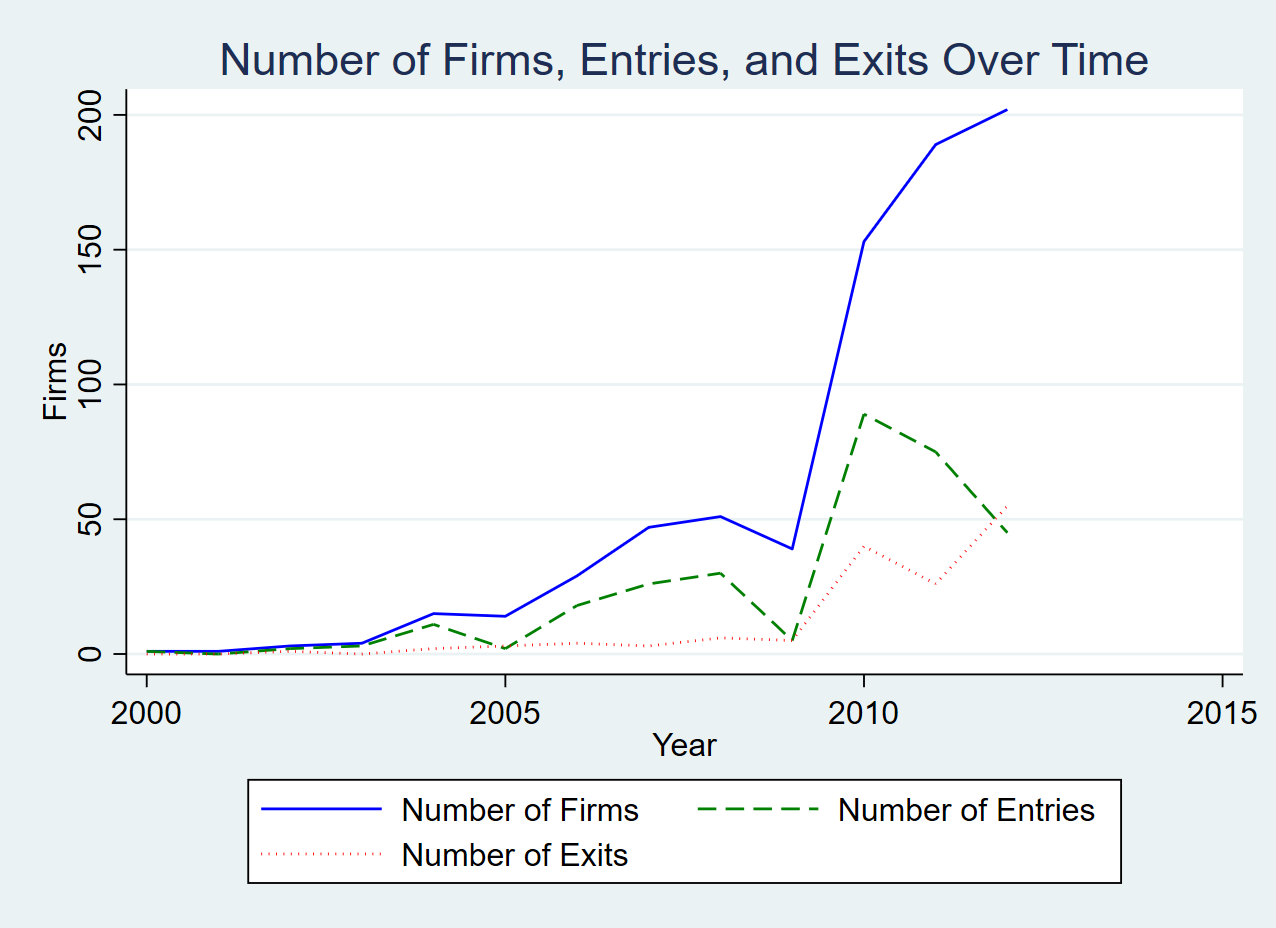
\includegraphics[width=0.6\linewidth]{Figures/Entry and Exit over time.png}
%         %\caption{Firms entered quickly at start, then exited relatively quickly}
%     \end{figure}
% \end{frame}

% \begin{frame}{Chinese firms: capital and investment increased over time and then dropped}
%     \begin{figure}
%         \centering
%         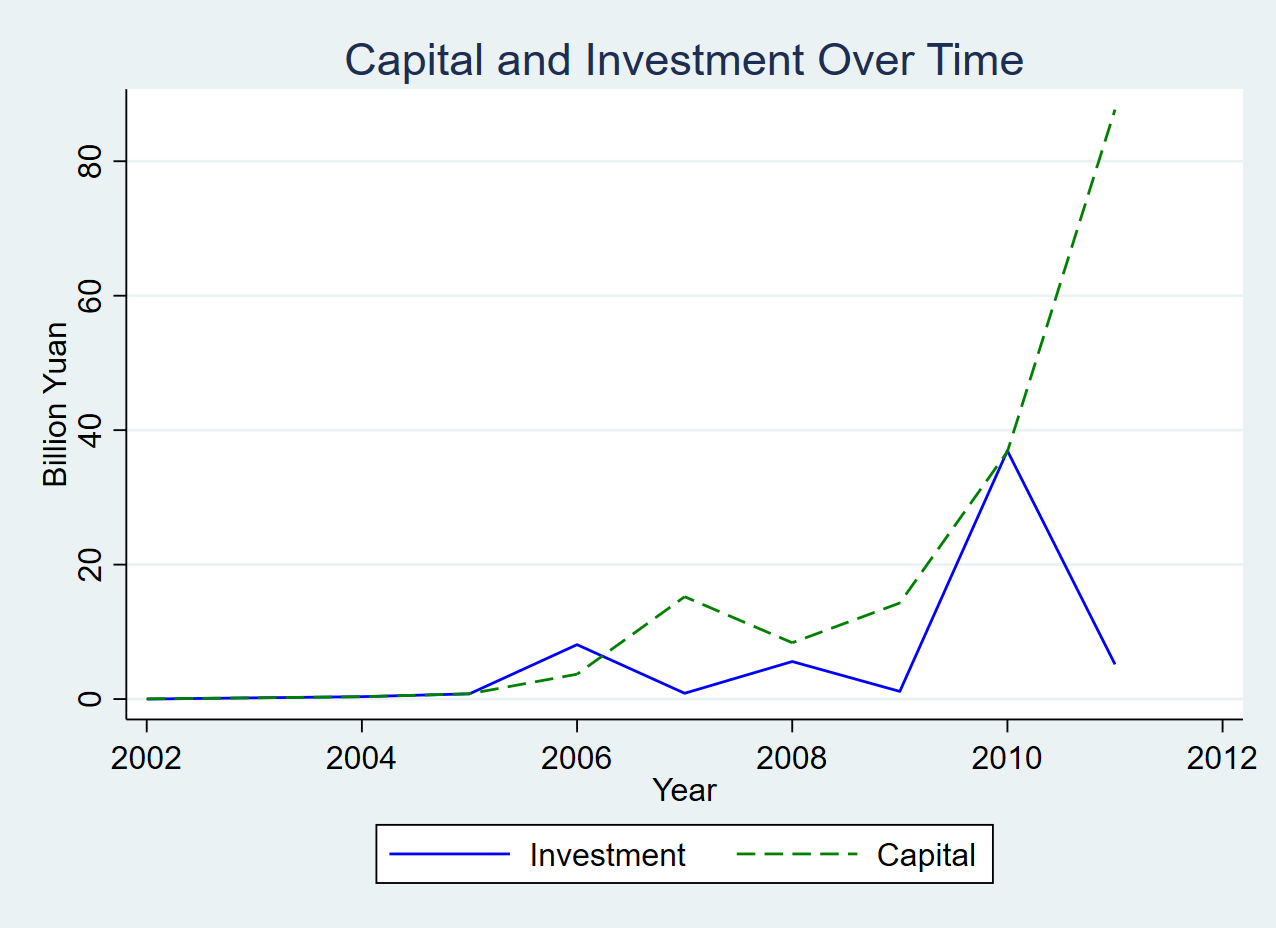
\includegraphics[width=0.6\linewidth]{Figures/Capital and Investment over Time.png}
%         %\caption{Capital and investment increased over time and then dropped}
%         \label{fig:enter-label}
%     \end{figure}
% \end{frame}

% % \begin{frame}{HHI has decreased as the industry has become less concentrated}
% %     \begin{figure}
% %         \centering
% %         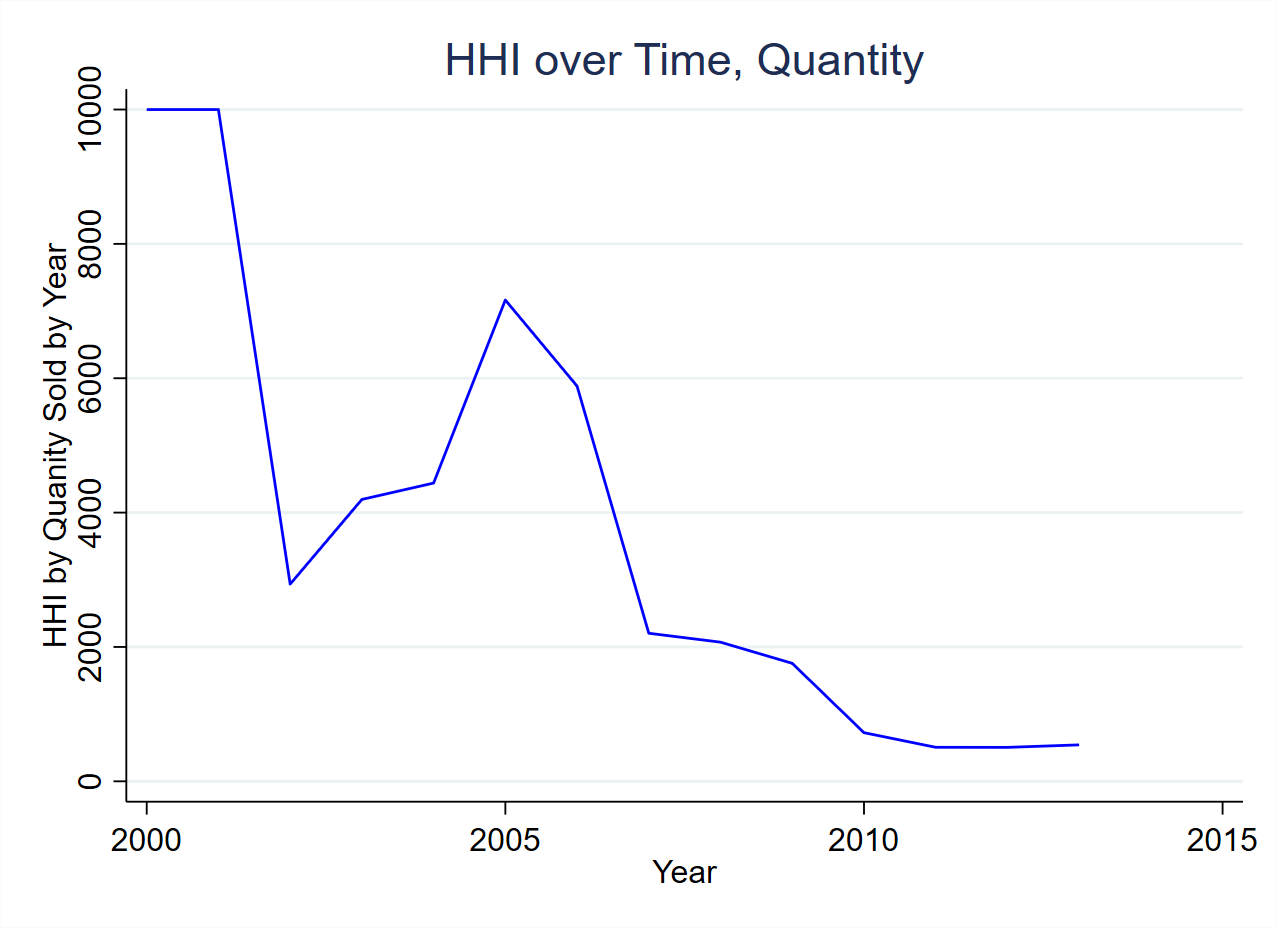
\includegraphics[width=.7\linewidth]{Figures/HHI by Quantity Sold by Year.png}
% %         %\caption{HHI has decreased as the industry has become less concentrated}
% %     \end{figure}
% % \end{frame}

% \begin{frame}{Summary Statistics of Chinese Firms}
%     \begin{table}[htbp]\centering
% \caption{Summary Statistics}
% \begin{tabular}{lcccc}
% \hline\hline
% Variable            & Mean         & Std. Dev.    & Min          & Max          \\
% \hline
% Age           & 5.49         & 5.44         & 0          & 48           \\
% Output        & 1.40 Billion    & 2.79 Billion    & 424,000    & 23.9 Billion    \\
% Inventory     & 157 Million    & 320 Million     & 0            & 3 Billion    \\
%  Capital       & 351 Million   & 693 Million     & 350,000      & 11 Billion     \\
% Sales         & 1.45 Billion     & 3.13 Billion     & 4,800        & 25.9 Billion     \\
% Investment          & 1.1 Million    & 837 Million    & -10.2 Billion    & 10.2 Billion     \\
% \hline
% Firm-years        & 754          &              &              &              \\
% \hline\hline
% \end{tabular}
% \end{table}
% \end{frame}


\section{Model}

\begin{frame}[plain, noframenumbering]
\begin{center} 
{\color{sbured}\LARGE II. Model}
\end{center}
\end{frame}

\begin{frame}{Model Timing}
\begin{itemize}
    \item Notations: firm $j$, year $t$, economic region $m$ (US, EU, Japan, China, India, ROW)
\end{itemize}
Every year $t$,
    \begin{enumerate}
        \item Incumbent firms observe production cost shock $\omega_{jmt}$, choose quantity $q_{jmt}$
        \item Incumbent firms observe investment cost shock $\nu_{jt}$, choose new investment $i_{jt}$
        \item Incumbent firms observe scrap value $\phi_{jt}$, decide on exit. Entrants observe entry shock $\kappa_{jt}$, decide on entry.
    \end{enumerate}
\end{frame}
% \begin{frame}{Model Timing}
% \begin{tikzpicture}[>=Stealth, node distance=1.5cm, every node/.style={scale=0.9, rectangle, draw, align=center, rounded corners}]

%     % Event 1
%     \node (event1) {Incumbent firms 
%     \\ see cost shock $\omega_{jmt}$
%     \\ choose quantity $q_{jmt}$};
    
%     % Arrow to Event 2
%     \draw[->] (event1.east) -- ++(1, 0) node[midway, above] {$t$};
    
%     % Event 2
%     \node[right=of event1] (event2) {Incumbent firms \\ choose investment};
    
%     % Arrow to Event 3
%     \draw[->] (event2.east) -- ++(1, 0);
    
%     % Event 3
%     \node[right=of event2] (event3) {Incumbent firms \\ exit, entrants \\ enter};
    
%     % Arrow for cycle restart
%     \draw[->, dashed] (event3.east) -- ++(1, 0) node[midway, above] {$t+1$};
    
%     % Cycle restart node
%     \node[right=of event3] (restart) {Cycle restarts};

% \end{tikzpicture}
% \end{frame}
\begin{frame}{Demand}
\begin{itemize}
   \item Aggregate inverse demand for solar panels:
        \begin{equation}
          Q_{mt}=Q_{m}(P_{mt},d_{mt})
        \end{equation}
    \begin{itemize}
        \item $P_{mt}$: price paid by consumers in region $m$ at time $t$; = $P_t$ $\times$ (1 + tariff$_{mt}$) - subsidy$_{mt}$
        \item $d_{mt}$: demand shifters
    \end{itemize}
 \end{itemize}

\end{frame}

\begin{frame}{Production}
\begin{itemize}
    \item Firm $j$'s marginal cost of shipping $q_{jmt}$ units to region $m$ at time $t$:
    \begin{align}
         MC^q_m(q_{jmt},s_{jt},\omega_{jmt}) \nonumber
    \end{align}
       
    \begin{itemize}
        %\item $F_{m}$: fixed cost of operation
        \item $s_{jt}$: firm characteristics (capital, age, location, ownership status), aggregate cost shifters affecting all firms (e.g. polysilicon price), policy dummies that capture the effect of industrial policies on production costs
        \item $\omega_{jmt}$: production cost shock
    \end{itemize}
\end{itemize}

\pause

\begin{itemize}
    \item Cournot competition with output satisfying FOC:
\end{itemize}
    \begin{equation}
    P_{mt}+q_{jmt}^*\frac{\partial P_{m}(Q_{mt},d_{mt})}{\partial q_{jmt}}=MC^q_m (q_{jmt}^*,s_{jt},\omega_{jmt}) \label{eq:foc_q}
    \end{equation}
\end{frame}

\begin{frame}{Firm Profit}
\begin{itemize}
\item Firm $j$'s expected profit before the production cost shocks are realized:
\[
\pi(s_{jt}) = \mathbb{E} [\sum_m \pi_m(s_{jt},\omega_{jmt})]
\]
where $\pi_m(s_{jt},\omega_{jmt})$ is firm $j$'s equilibrium profit in region $m$
%\item In each period, global price $P_t$ equates aggregate demand and supply, where the aggregate supply is the sum of $q_{jmt}^*$ defined in (3)
\end{itemize}
\end{frame}

\begin{frame}{Incumbents: Investment and Exit}
\begin{itemize}
    \item Draws a scrap value $\phi_{jt}$ from the distribution $F_\phi$ and decides whether to exit
    \item If active, draws an investment cost shock $\nu_{jt}$ from a distribution $F_\nu$ and chooses investment $i_{jt}$ at cost $C^i(i_{jt},s_{jt},\nu_{jt})$
    \item Ex-post value function:
    \begin{align}
        V(s_{jt},\phi_{jt})&=\pi(s_{jt})+\max\{\phi_{jt},\mathbb{E}[\max_i\{-C^i(i,s_{jt},\nu_{jt})+\beta \mathbb{E}[V(s_{jt+1})|s_{jt},i]\}]\} \nonumber \\
           &=\pi(s_{jt})+\max\{\phi_{jt},CV(s_{jt})\}  \label{eq:incumbent_value_fn} \\
        CV(s_{jt}) & \equiv \mathbb{E}[-\{C^i(i^*,s_{jt},\nu_{jt})+\beta \mathbb{E}[V(s_{jt+1})|s_{jt},i^*]] \nonumber
    \end{align}
\end{itemize}
    
\end{frame}

\begin{frame}{Incumbents: Investment and Exit}
\begin{itemize}
\item Probability of exit:
    \begin{align}
        p^x(s_{jt}) & \equiv Pr(\phi_{jt} > CV(s_{jt})) = 1-F_\phi(CV(s_{jt})) \label{eq:exit_policy_fn}
    \end{align}

\item Optimal investment $i^*=i^*(s_{jt},\nu_{jt})$ satisfies FOC:
    \begin{align}
        \beta\frac{\partial \mathbb{E}[V(s_{jt+1})|s_{jt},i]}{\partial i} &\leq \frac{\partial C^i(i,s_{jt},\nu_{jt})}{\partial i} \label{eq:investment_policy_fn}
    \end{align}

\item Marginal investment cost:
   \begin{align}
       MC^i(i_{jt},s_{jt},\nu_{jt}) & = s_{jt} \kappa_1 + \kappa_2 i_{jt} + \kappa_3 \nu_{jt} \label{eq:investment_cost}
    \end{align} 
\end{itemize}
    
\end{frame}

\begin{frame}{Potential Entrants: Entry}
\begin{itemize}
    \item $\bar N$ potential entrants draw entry cost $\kappa_{jt}$ from distribution $F_\kappa$ and decide on entry
    \item Potential entrant $j$'s problem:
    \begin{align}
       & \max\{0,-\kappa_{jt}+\mathbb{E}[-C^i(s_{jt})+\beta \mathbb{E}[V(s_{jt+1})|s_{jt}]]\} \\
       VE(s_{jt}) & \equiv \mathbb{E}[-C^i(s_{jt})+\beta \mathbb{E}[V(s_{jt+1})|s_{jt}]]\} \nonumber
    \end{align}

    \item Probability of entry:
    \begin{align}
        p^e(s_{jt}) & \equiv Pr(\kappa_{jt}\leq VE(s_{jt})) = F_\kappa(VE(s_{jt})) \label{eq:entry_policy_fn}
    \end{align}

\end{itemize}
\end{frame}

\begin{frame}{Markov-Perfect Equilibrium}
\begin{itemize}
    \item Production quantity $q_{jmt}^*$ satisfies (\ref{eq:foc_q})
    \item Investment policy function $i^*(s_{jt},\nu_{jt})$ satisfies (\ref{eq:investment_policy_fn})
    \item Exit policy function $p^x(s_{jt})$ satisfies (\ref{eq:exit_policy_fn})
    \item Entry policy function $p^e(s_{jt})$ satisfies (\ref{eq:entry_policy_fn})
    \item Price $P_t$ clears the market so that aggregate demand equals aggregate supply
    \item Incumbent's value function $V(s_{jt})$ satisfies (\ref{eq:incumbent_value_fn})
\end{itemize}
\end{frame}


\section{Estimation Strategy}
\begin{frame}[plain, noframenumbering]
\begin{center} 
{\color{sbured}\LARGE III. Estimation Strategy}
\end{center}
\end{frame}

% \begin{frame}{Estimation Strategy: Overview}
% \begin{itemize}
%     \item Static parameters
%     \item Dynamic parameters
% \end{itemize}
% \end{frame}


\begin{frame}{Static Parameters: Demand}
    \begin{itemize}
    \item Linear demand specification:
    \[
    Q_{mt}=\alpha_{m} P_{mt}+d_{mt}\beta_{m}+\epsilon_{mt} \nonumber
    \]
        \begin{itemize}
        \item $Q_{mt}$: total capacity installed by region / quarter
        \item $P_{mt}$: Global price adjusted for local tariffs and subsidies
        \item $d_{mt}$: demand shifters include electricity consumption, feed-in tariff, GDP, region FEs, time FEs
        \end{itemize}
    \item IV for global price: polysilicon price and production
    \end{itemize}
\end{frame}

\begin{frame}{Static Parameters: Production Cost}
\begin{itemize}
     \item Marginal cost function:
    \begin{equation}
        MC_m(q_{jmt},s_{jmt},\omega_{jmt})=\gamma_{m}^0+\gamma_m^q q_{jmt}+\gamma^s s_{jt}+\omega_{jmt}  \nonumber
    \end{equation}

   \begin{itemize}
       \item $q_{jmt}$: units produced by firm $j$ to region $m$ in period $t$
       \item $s_{jt}$:  cost  shifters include  input prices, capital, employment, ownership status, province, inventory, and time period dummies
       \item $\omega_{jmt}$: product cost shock $\sim N(0,\sigma^2_\omega)$
   \end{itemize}
\end{itemize}
\end{frame}

 \begin{frame}{Static Parameters: Production Cost}
\begin{itemize}   
    \item FOC of Cournot competition:
    \begin{align}
        q_{jmt}^*&=\frac{P_{mt}-\gamma_m^0-q_{jmt}-s_{jt}\gamma^s-\omega_{jmt}}{\gamma_m^q-\alpha_m} \nonumber \\
        q_{jmt}&=max(0,q_{jmt}^*)
    \end{align}
    \pause
    \item Tobit model:
    \begin{align}
    L(\gamma)&=\prod_{j,m,t;q_{jmt}=0} Pr(q_{jmt}=0|s_{jt};\gamma)\times\prod_{j,m,t;q_{jmt}>0} f_{q}(q_{jmt}|s_{jt};\gamma)
    \end{align}

\end{itemize}
\end{frame}

\begin{frame}{Dynamic Parameters: BBL two-stage}

\begin{itemize}
    \item First stage: 
        \begin{itemize}
        \item Non-parametrically estimate policy functions (investment, exit, entry)
        \item Estimate state transition process
        \item Approximate the value functions
        \end{itemize}
    \item Second stage: MLE estimate the dynamic parameters

\end{itemize}


\end{frame}
\begin{frame}{First Stage: Exit Policy Function}
\begin{itemize}
    \item Assume scrap value follows a normal  distribution
    \item Exit function estimated as probit of flexible polynomial of states $s_{jt}$
    \begin{equation}
        Pr(\chi_{jt}=1|s_{jt})=\Phi(h(s_{jt}))
    \end{equation}

    \end{itemize}
\end{frame}

\begin{frame}{First Stage: Investment Policy Function}
\begin{itemize}
    \item Under reasonable assumptions, the optimal investment $i^*(s_{jt},\nu_{jt})$ is monotonically decreasing in investment shock $\nu_{jt}$.
        \begin{align}
        i^*|s_{jt} &= G^{-1}(1-F_{\nu}(\nu\mid s_{jt})) \label{eq:est_investment}
         \end{align}
         where 
         \begin{itemize}
             \item $G(i\mid s_{jt})$: empirical distribution of  investment given the state variables
             \item $F_{\nu}(\nu\mid s_{jt})$: the assumed distribution of $\nu$ conditional on state variables
         \end{itemize}
     \item Assume $\nu_{jt} \sim $ standard normal, independent of $s_{jt}$ and enters additively
        \begin{align}
        i_{jt}^* &= h_1(s_{jt})+h_2(\nu_{jt})
        \end{align}
     \item Regress $i_{jt}$ on $s_{jt}$ to get $h_1(s_{jt})$ and $i_{jt}-\hat h_1(s_{jt})$; then estimate $h_2$ using (\ref{eq:est_investment})
        
\end{itemize} 
\end{frame}

\begin{frame}{First Stage: State Space}
\begin{itemize}
%\item High-dimensional state space $s_{jt}$ 
\item Assumption: firms do not keep track of the state variables of every rival and use industry-level prices as a sufficient statistic, similar to the oblivious equilibrium concept  (Weintraub et al (2008), Benkard et al (2015))
\item $s_{jt}$  enters MC linearly $\Longrightarrow$ collapse them into a one-dimensional index $\bar s_{jt} = -s_{jt} \hat \gamma^s$
\item Capital depreciates at rate $\delta = 2.3\%$
\[
k_{jt+1}  = (1-\delta) k_{jt} + i_{jt}
\]
\item Polysilicon price: AR(1), different processes before \& after 2009
\item Solar panel price: AR(1), different processes before \& after 2009
\item Government policies are perceived permanent 
\end{itemize} 
\end{frame}

\begin{frame}{First Stage: Value Function}
\begin{itemize}
    \item Scrap value $\phi_{jt} \sim $ exponential ($1/\sigma_\phi$)
    \item Ex-ante value function:
    \begin{align}
        V(s_{jt}) & = \mathbb{E}_\phi[\pi(s_{jt}) + max\{\phi_{jt},CV(s_{jt})\}] \nonumber \\
        & = \pi(s_{jt}) + p^x(s_{jt}) \sigma_\phi + CV(s_{jt})
    \end{align}
    \item B-spline basis function to approximate $V(s_{jt})$: Sweeting (2013)
\end{itemize}
\end{frame}

\begin{frame}{Second Stage: MLE [1]}
\begin{itemize}
    \item Dynamic parameters: $\theta = (\sigma_\phi, \kappa)$
       \begin{align}
        max_\theta L(\theta) & = \sum_{jt} log(f(\chi_{jt};\theta)) + \sum_{jt} log(g(i_{jt};\theta)) \nonumber \\
        s.t. \ V(s_{jt};\theta) & = \pi(s_{jt}) + p^x(s_{jt}) \sigma_\phi + CV(s_{jt};\theta)  \nonumber
        \end{align}
     \item $f(\chi_{jt};\theta)$: Prob. of exit
     \item $g(i_{jt};\theta)$: Density of investment
\end{itemize}
\end{frame}

\begin{frame}{Second Stage: MLE [2]}
\begin{itemize}
    \item The log-likelihood for exit:
    \begin{align}
        \sum_{jt} log(f(\chi_{jt})) &= \sum_{jt} \Big[ (1-\chi_{jt}) log(1-exp(-\frac{CV(s_{jt})}{\sigma_\phi})) - \chi_{jt} \frac{CV(s_{jt};\theta)}{\sigma_\phi} \Big]
    \end{align}
    \item The likelihood of positive investment: 
    \begin{align}
        g(i_{jt}) &= \frac{f_\nu(\nu_{jt})}{\partial i^*(s_{jt},\nu_{jt}) /\partial \nu_{jt}}
    \end{align}
    \item The likelihood of non-positive investment: 
    \begin{align}
        g(i_{jt}) &= Pr\Big( [\beta\frac{\partial \mathbb{E}[V(s_{jt+1})|s_{jt},i]}{\partial i} - \frac{\partial C^i(i,s_{jt},\nu_{jt})}{\partial i}]_{i=0} \leq 0  \Big)
    \end{align}
\end{itemize}
\end{frame}
% \section{Estimation Results}
% \begin{frame}[plain, noframenumbering]
% \begin{center} 
% {\color{sbured}\LARGE V. Estimation Results}
% \end{center}
% \end{frame}


% \begin{frame}{Estimation Results: Demand}
% \begin{table}[ht]
% \centering
% %\caption{Demand Function Results}
% %\label{tab:regression_results}
% \scriptsize  % Reduce font size to scriptsize
% \renewcommand{\arraystretch}{0.5}  % Reduce space between rows
% \resizebox{!}{0.35\textheight}{\begin{tabular}{l S[table-format=-1.3]}
% \toprule
% \textbf{Variables} & \textbf{Model} \\
% \midrule
% Constant         & 56.7\sym{***} \\
% %                 & (3.75) \\
% Price India & -.166\sym{***} \\
% %                 & (-4.18) \\
% Price ROW & -7.92\\
% %                 & (-1.59) \\
% Price China & -6.59\sym{**} \\
% %                 & (-2.16) \\
% Price Japan & -6.41\sym{*} \\
% %                 & (-1.74) \\
% Price EU & -9.03 \sym{**} \\
% %                 & (-2.5) \\
% Price United States              & -7.15\sym{**} \\
% %                 & (-2.51) \\
% Electricity Consumption          & -3.15 \sym{**} \\
% %                 & (-3.16) \\
% Feed-in Tariff          & .5612 \\
%  %                & (.03) \\
% Theoretical Potential       & -5.19 \\
%  %                & (-.81) \\
% GDP & 1.31\sym{*} \\
% %                 & (1.82) \\
% After 2009 & -28\sym{**} \\
% %                 & (-2.63) \\
% \midrule
% \textbf{Observations} & 138 \\
% \bottomrule
% \end{tabular}}
% \end{table}
% \end{frame}

% \begin{frame}{Estimation Results: Marginal Cost}
%     \begin{table}[ht]
% \centering
% %\caption{Marginal Cost Results}
% %\label{tab:regression_results}
% \scriptsize  % Reduce font size to scriptsize
% \renewcommand{\arraystretch}{0.5}  % Reduce space between rows
% \resizebox{!}{0.35\textheight}{\begin{tabular}{l S[table-format=-1.3]}
% \toprule
% \textbf{Variables} & \textbf{Model} \\
% \midrule
% Constant         & 17.46\sym{***} \\
% %                 & (21.01) \\
% Quantity & -3.16\sym{**} \\
%  %                & (-2.64) \\
%  Price of Polysilicon & 1.14\sym{***} \\

% Capital & -2.23\sym{***} \\
% %                 & (5.75) \\
% Capital Squared & 1.9\sym{***} \\
%  %                & (3.81) \\
% Employment       & -3\sym{**} \\
%  %                & (-3.37) \\
% Inventory & -9.29 \\
%  %                & (-1.85) \\
% Age              & -.510\sym{***} \\
%   %               & (-13.57) \\
% Foreign          & -.557 \\
%  %                & (-.79) \\
% Private          & -1.42\sym{*} \\
% %                 & (-2.00) \\
% Large Firm       & -4.58\sym{*} \\
%  %                & (-2.45) \\
% Province: Zhejiang & .271 \\
%    %              & (.47) \\
% Province: Jiangsu & .35 \\
%  %                & (-0.63) \\
% Province: Guangdong & 1.039 \\
% %                 & (0.72) \\

% \midrule
% \textbf{$\sigma_u$}    & 8.615\sym{***} \\
%  %                & (30.05) \\
% \textbf{$\sigma_e$}    & 4.659\sym{***} \\
% %                 & (50.28) \\
% \midrule
% \textbf{Observations} & 1964 \\
% \bottomrule
% \end{tabular}}

% \end{table}
%\end{frame}

% \begin{frame}{Exit Probit Function}
%     \begin{table}[ht]
% \centering
% %\caption{Exit Probit Results}
% %\label{tab:regression_results}
% \scriptsize  % Reduce font size to scriptsize
% \renewcommand{\arraystretch}{0.5}  % Reduce space between rows
% \resizebox{!}{0.35\textheight}{\begin{tabular}{l S[table-format=-1.3]}
% \toprule
% \textbf{Variables} & \textbf{Model} \\
% \midrule
% Constant         & -1.4\sym{***} \\
% %                 & (-3.54) \\
% Price & 7.79 \\
% %                 & (1.00) \\
% $\bar{S}$ & 1.14 \\
%  %                & (.44) \\
% Price Polysilicon & -2.53 \\
% %                 & (-1.25) \\
% Inventory       & -1.84 \\
%  %                & (-.68) \\
% After 2009 & .505 \\
% %                 & (1.8) \\
% \midrule
% \textbf{$\sigma_u$}    & .3627 \\
%  %                & (30.05) \\
% \midrule
% \textbf{Observations} & 612 \\
% \bottomrule
% \end{tabular}}
% \end{table}
% \end{frame}

% \begin{frame}{Investment Policy Function Results}
%     \begin{table}[ht]
% \centering
% %\caption{Investment Results}
% %\label{tab:regression_results}
% \scriptsize  % Reduce font size to scriptsize
% \renewcommand{\arraystretch}{0.5}  % Reduce space between rows
% \resizebox{!}{0.35\textheight}{\begin{tabular}{l S[table-format=-1.3]}
% \toprule
% \textbf{Variables} & \textbf{Model} \\
% \midrule
% Constant         & -1.47\sym{***} \\
%                  & (-4.24) \\
% bspline Capital 1 & -4.47\sym{**} \\
%                  & (-2.8) \\
% bspline Capital 2 & 8.07 \\
%                  & (.79) \\
% $\bar{S}$ & 3.37 \\
%                  & (-1.43) \\
% Price       & 2.6\sym{***} \\
%                  & (3.7) \\
% Price Polysilicon & -2.8 \\
%                  & (-1.79) \\
% After 2009              & 5.84\sym{**} \\
%                  & (2.62) \\
% \midrule
% \textbf{$\sigma_u$}    & 1.15\sym{***} \\
%                  & (7.21) \\
% \textbf{$\sigma_e$}    & 1.09\sym{***} \\
%                  & (18) \\
% \midrule
% \textbf{Observations} & 610 \\
% \bottomrule
% \end{tabular}}
% \end{table}
% \end{frame}

\section{Next Steps}
\begin{frame}{Next Steps}
    \begin{itemize}
        \item Estimate demand and MC
        \item Estimate policy functions
        \item Approximate value function
        \item Second stage of BBL: MLE of dynamic parameters
        \item CFs
    \end{itemize}
\end{frame}
%----------------------------------------------------
\end{document}
